\section{Experiment}
\label{sec:exp}
% We have conducted a comprehensive experimental evaluation on the
% performance of \name and also compared \name with other closely
% related systems.

\subsection{Experiment Setup}
\label{sec:setupexp}
All experiments are conducted on a cluster consisting of 10 nodes with
two configurations: (1) 8 machines with a 6-core Intel Xeon E5-2603 v3
1.60GHz processor and 20GB RAM; (2) 2 machines with a 6-core Intel
Xeon E5-2620 2.00GHz processor and 56GB RAM. Each node is connected to
a Gigabit Ethernet switch and runs Ubuntu 14.04.2 LTS with Hadoop
2.4.1 and Spark 1.3.0. We select one machine of type (2) as the master
node and the rest are slave nodes. The Spark cluster is deployed in
standalone mode and configured to use up to 15GB memory on each slave
node. We used the following real and synthetic datasets: \vspace{-1mm}
\begin{pkl}
\item OSM: OSM is a real dataset extracted from the OpenStreetMap
  project \cite{osm}.  We took uniform random samples of various size
  (1 million to 1 billion records) from the complete OSM data set and
  used them in our experiments. Each record contains a rid,
  2-dimensional coordinate, time stamp and description.
  \dong{new experiments rely on only rid and two coordinates.}
\item GDELT: GDELT stands for Global Data on Events, Language and Tone
  \cite{gdelt}, which is an open database of human society, containing
  75 million records in total. In our experiment, each record takes 7
  attributes: a timestamp, and three 2-dimensional coordinates which
  represent the locations for the start, the terminal, and the action
  of an event.
\item RC: We also generated synthetic datasets of various sizes (1
  million to 1 billion records) and dimensions (2 - 6 dimensions)
  using a {\em random cluster} generator with Gaussian
  distributions. Each record in $d$-dimension contains $d+1$
  attributes: namely, a record ID and its spatial coordinates.
\end{pkl}\vspace{-2mm}

For single-relation operations (i.e. range and $k$NN queries), we
evaluate the performance with two metrics: {\em throughput and
  latency}. In particular, for both \name and Spark SQL, we run a
Spark instance with thread pool size = 10 in the driver program, and
issue 500 queries to the system to calculate the throughput. For other
systems that we reviewed in Section \ref{sec:background}, since they
do not use a multi-threading model, we submit 20 queries at the same
time, and run them as 20 different processes to ensure full
utilization of the cluster resource. The throughput is calculated by
dividing the total number of queries over the running time. Note that
this follows the same way these systems had used to measure their
throughput \cite{spatialhadoop}.  For all systems, we used 100
randomly generated queries to measure the average query latency.

For join operations, we focus on the average running time of a join
query over 10 randomly generated join queries for all systems.

In all experiments, HDFS block size is 64MB. By default, $k=10$ for a
$k$NN or a $k$NN join query. A range query is characterized by its
{\em query area, as a percentage over the entire area} that data
locate at. The default for range queries is $0.01\%$. The default
distance threshold $\tau$ for a distance join is set to $5$ (each
dimension is normalized into a domain from $0$ to
$1000$).% the area for a
% circle with radius $\tau=x$ retrieves roughly $y$ number of points
% {\em on average} from the second table.  $0.00005\%$ of the entire
% area.
The default partition size is is $500\times 10^3$ (500k) records per
partition. The default data set size for single-relation operations is
500 million records on OSM and 700 million on synthetic data sets, and
3 million records in each input table for a join. The default
dimensionality is 2.

%\feifei{Specify $x$ and $y$ above.}


% , and $3\times10^4$
% records.% Expected partition size for table indexing is $5\times10^5$ records
% by default, while that for joins is $3\times10^4$ records.

% \dong{We should not set default values on sample rate and expected
%   partition size here since we claim that \name will automatically
%   tune these configurations.}


\subsection{Cost of Indexing}
\label{sec:indexexp}
We first investigate the cost of indexing in \name and other
cluster-based spatial analytics systems, including SpatialSpark
\cite{spatialspark}, SpatialHadoop \cite{spatialhadoop}, and Hadoop
GIS \cite{hadoopgis}. Figure \ref{fig:index_datasize} presents the
index construction time in different systems on OSM data, when OSM
varies from 30 million to 1 billion records. As shown in the figure,
\name has the best performance among all systems and scales linearly
to the size of the data as well. For example, \name builds its index
(which uses R-tree for both local indexes and the global index) over
1 billion records, 60GB in file size, in around 25 minutes, which is
2.5x faster than SpatialHadoop, 3x faster than SpatialSpark, and 12x
faster than Hadoop GIS. Note that GeoSpark is faster than all of
other systems because it only uses Spark's default partitioner
without spatial locality and build local indexes on each partition,
thus does not involve data repartitioning and global indexing. Compared
to Hadoop based systems, \name indexes RDDs, while Hadoop-based systems
index HDFS file blocks. Even though SpatialSpark also uses Spark, but
it {\em does not} index RDDs natively. Instead, it indexes files in HDFS
as well.


%We do not include the result of GeoSpark because
%it only supports local indexing and does not provide a spatial RDD
%partitioner according to its latest open-sourced version (0.2.0).
%Thus, we are unable to compare it with other systems which has
%full support on data partition, local indexing and global indexing.


\begin{figure}[t]
	\centering
	\subfigure[Effect of data size (OSM).]{
		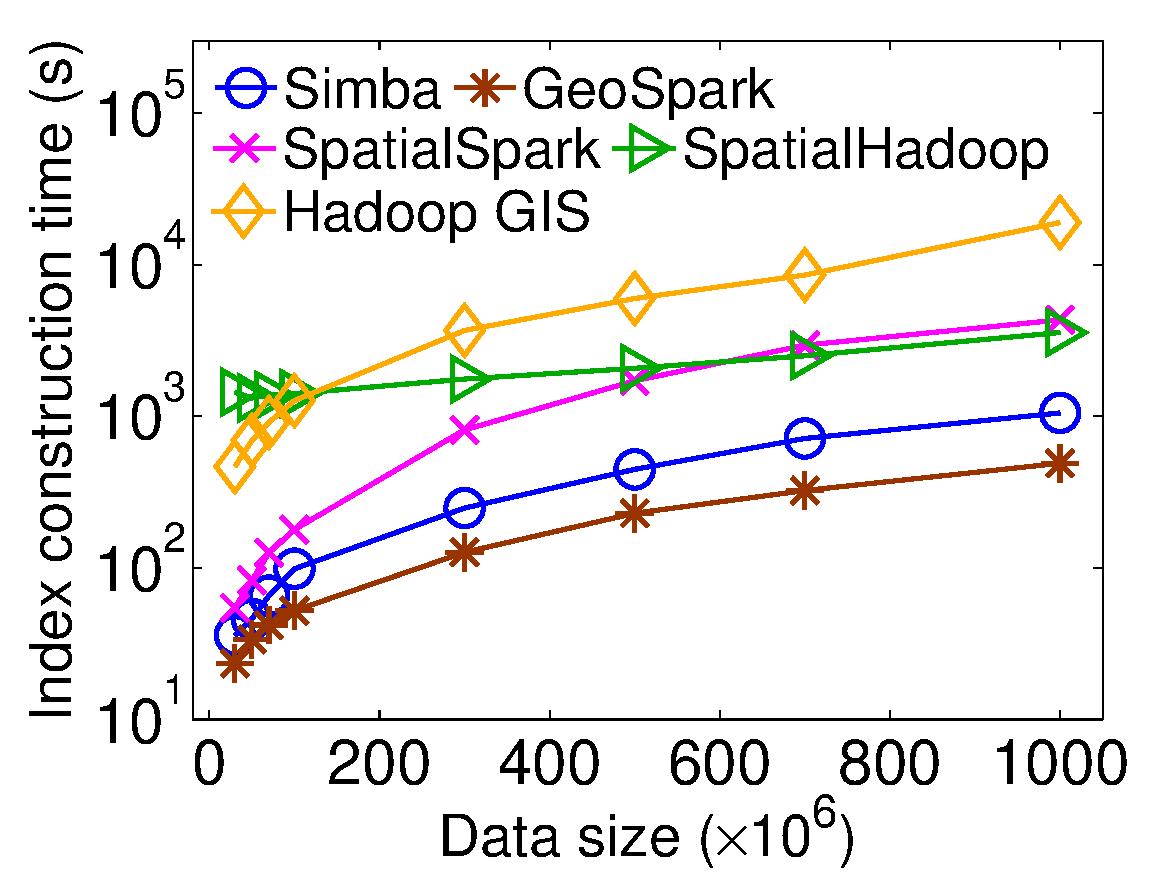
\includegraphics[width=1.55in]{figs/exp/index_time}
		\label{fig:index_datasize}}%\vspace{3mm}
	% \subfigure[Effect of partition size.]{
	% 	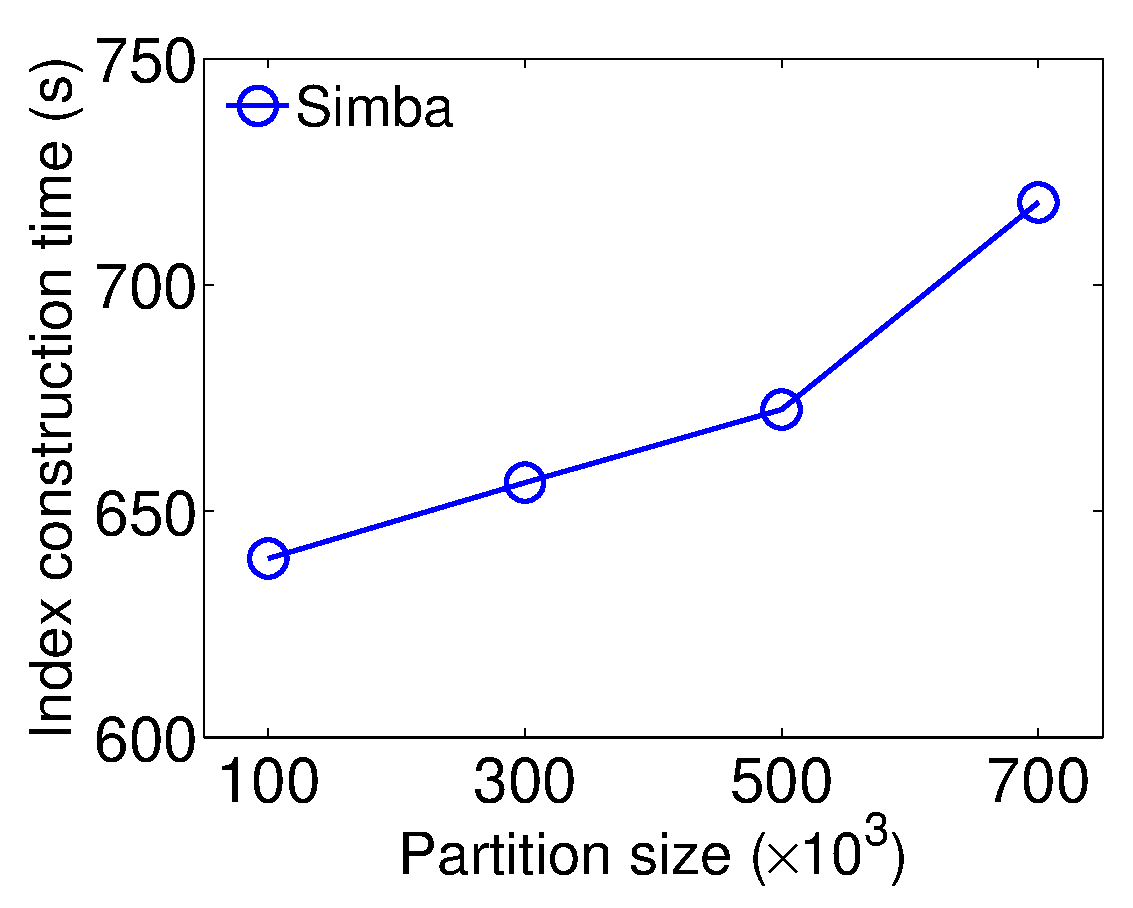
\includegraphics[width=1.55in]{figs/exp/osm_index_partsize_time}
	% 	\label{fig:index_partsize}}
	\subfigure[Effect of dimensionality.]{
		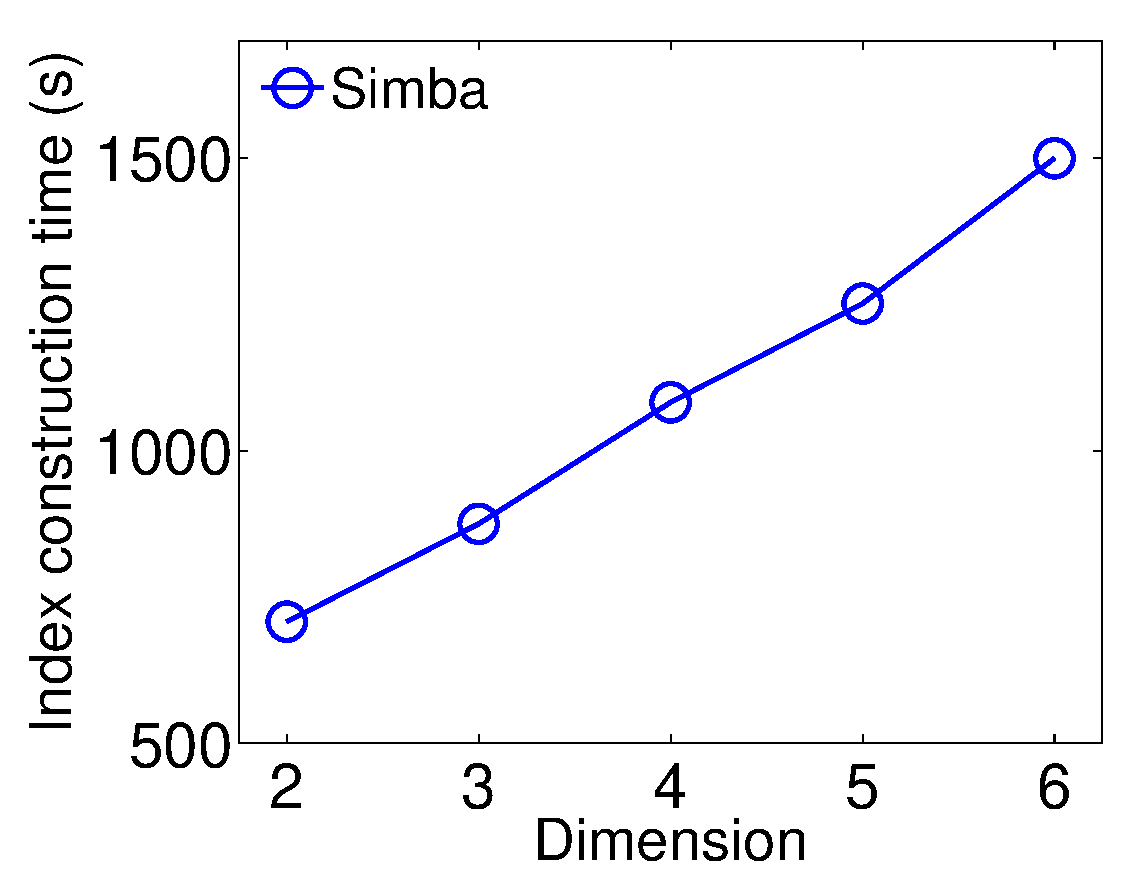
\includegraphics[width=1.55in]{figs/exp/index_dim_time}
		\label{fig:index_dim}}
	\caption{Index construction cost.}\vspace{-4mm}
	\label{fig:indexexp}
\end{figure}

We then investigated \name's index support in higher
dimensions. Figure \ref{fig:index_dim} shows the index construction
time in \name against number of dimensions on the synthetic data
set. The cost increases linearly with the increase in
dimensionality. Note that all {\em other systems can only support up
  to 2 dimensions}.


% Figure \ref{fig:index_partsize} shows that its index construction cost
% grows roughly linearly with respect to (wrt) partition size. This is
% because it is more costly to build local indexes over larger
% partitions (which outweighs the savings resulted from processing less
% number of partitions). % Note that We only show results for
% % \name since expected partition sizes for other systems are fixed to
% % the HDFS block size.


% \begin{figure}[t]
%     \centering
%     \begin{minipage}{1.60in}
%         \centering
%         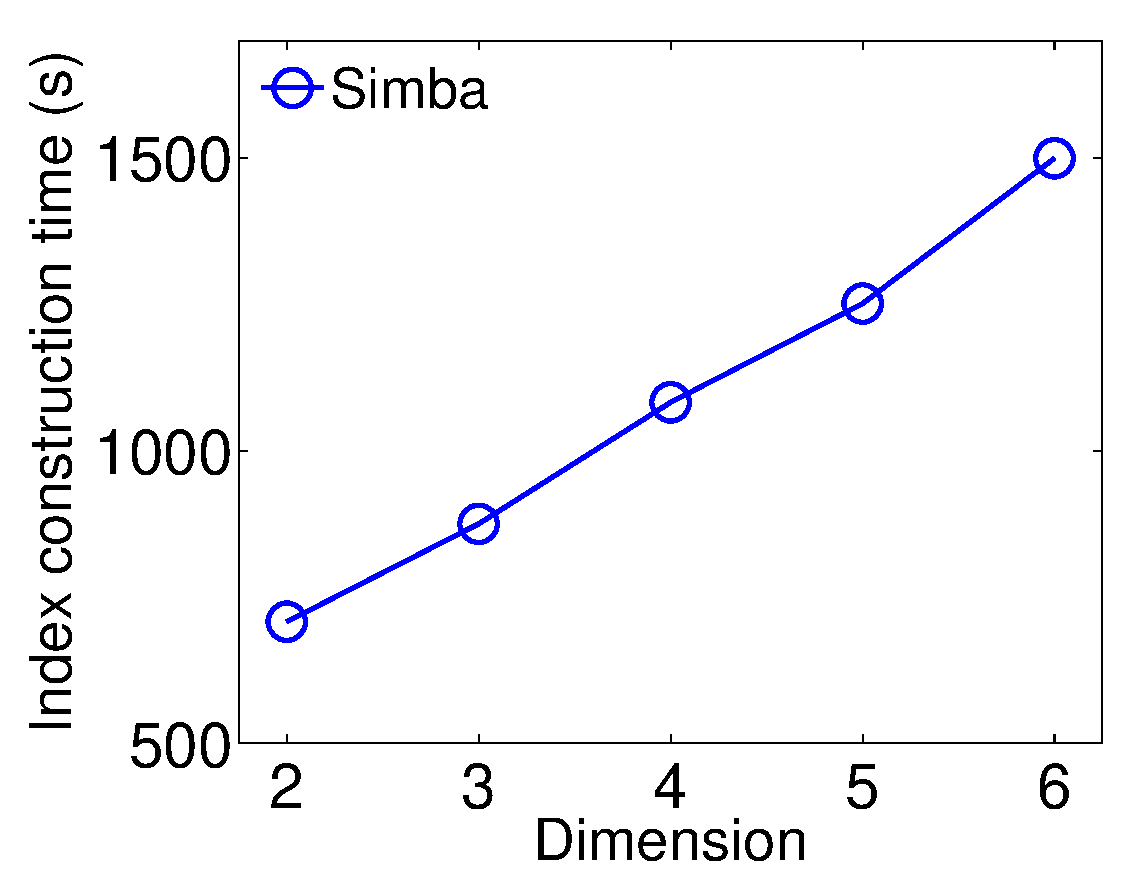
\includegraphics[width=1.50in]{figs/exp/index_dim_time}\vspace{-4mm}
%         \caption{Effect of dimensionality for index construction.}
%     		\label{fig:index_dim}
%     \end{minipage}
%     \hfill
%     \begin{minipage}{1.60in}
%       \centering
%       \vspace{0.5mm}
%       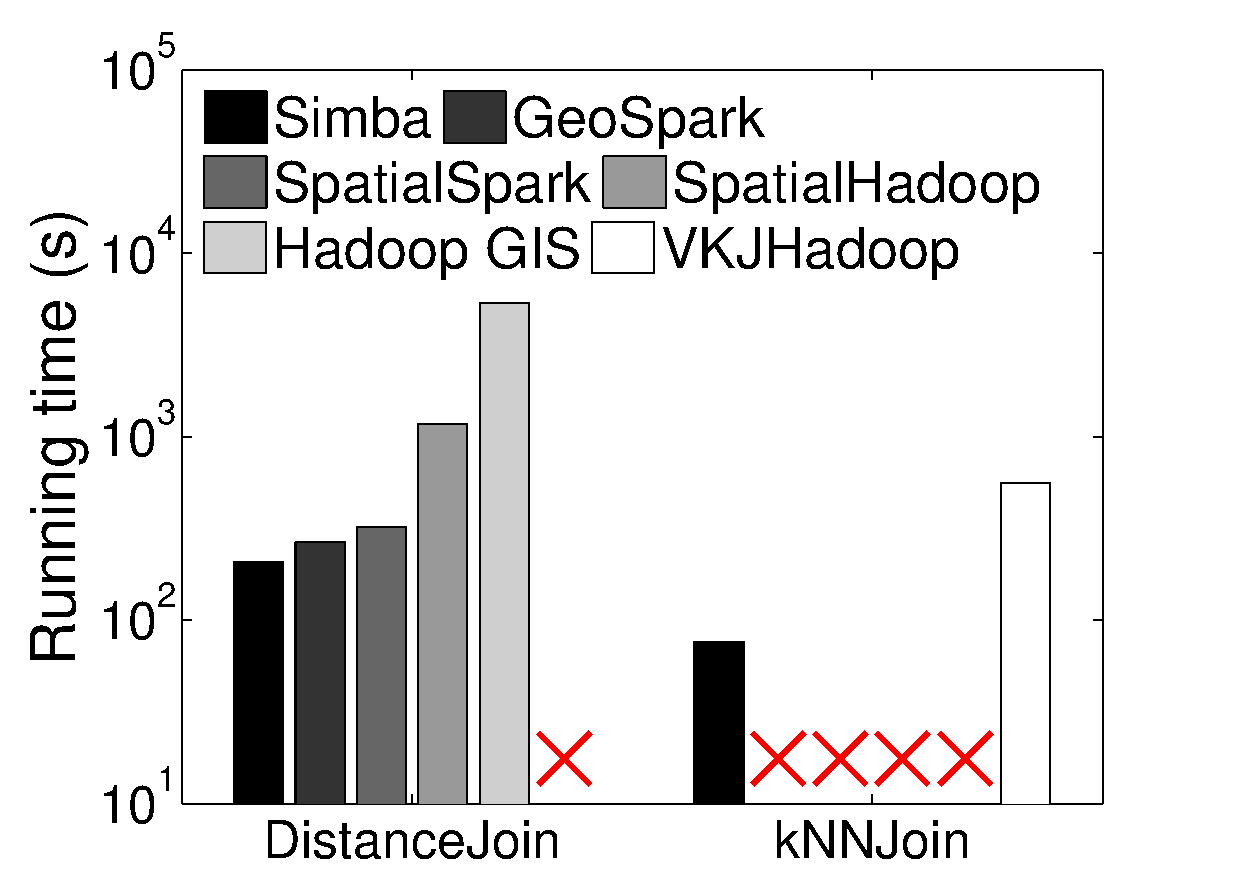
\includegraphics[width = 1.60in]{figs/exp/osm_join_time}\vspace{-2mm}
%       \caption{Join operations on different systems.}
%       \label{fig:system_join}
%     \end{minipage}
%     \vspace{-4mm}
% \end{figure}


\begin{figure}[!t]
	\subfigure[Throughput]{
		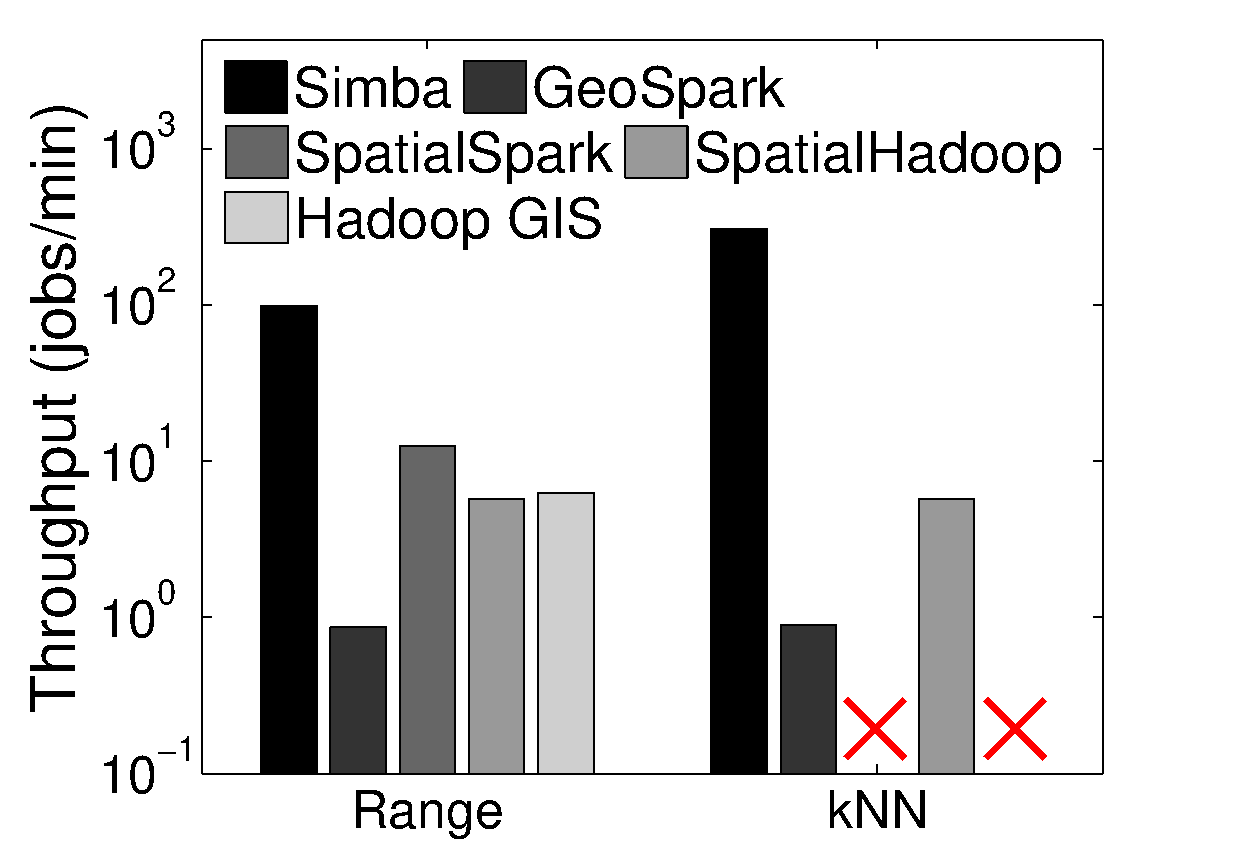
\includegraphics[width=1.55in]{figs/exp/osm_throughput_2}
		\label{fig:system_single_throughput}}
	\subfigure[Latency]{
		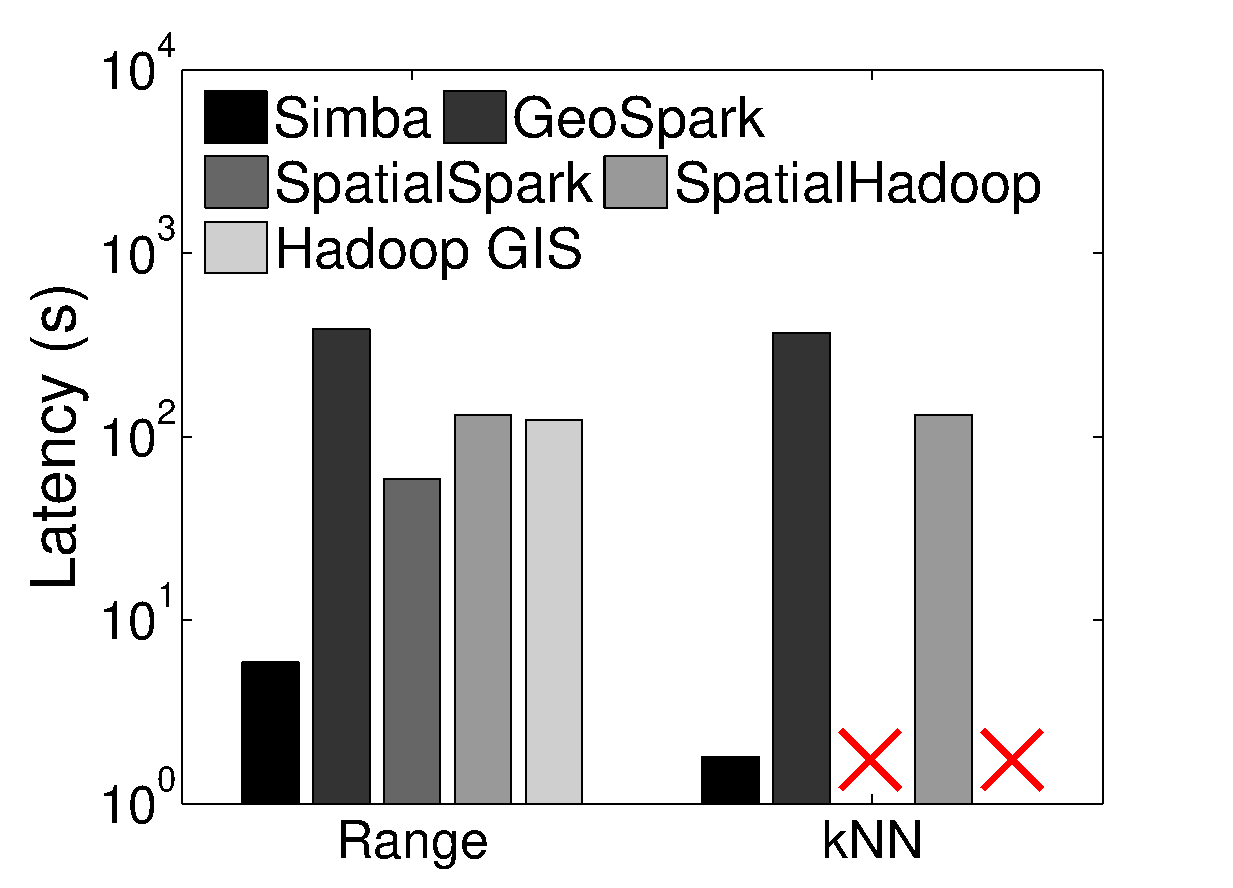
\includegraphics[width=1.55in]{figs/exp/osm_latency_2}
		\label{fig:system_single_latency}}
      \caption{Single-relation operations on different
        systems.}
	\label{fig:system_single}\vspace{-4mm}
\end{figure}

\subsection{Comparison with Existing Spatial Analytics Systems}
\label{sec:comparison}
In this section, we run all spatial operations supported by a system
with the default settings described in Section \ref{sec:setupexp} over
the default OSM dataset (500 million records in 30GB) on \name,
GeoSpark, SpatialSpark, SpatialHadoop, and Hadoop GIS, to compare their
performance.  A red cross mark in the following bar charts indicates
that the corresponding operation is {\em not supported} in a system.


%\vspace{-2mm}
%\begin{figure}[!h]
%	\centering
%	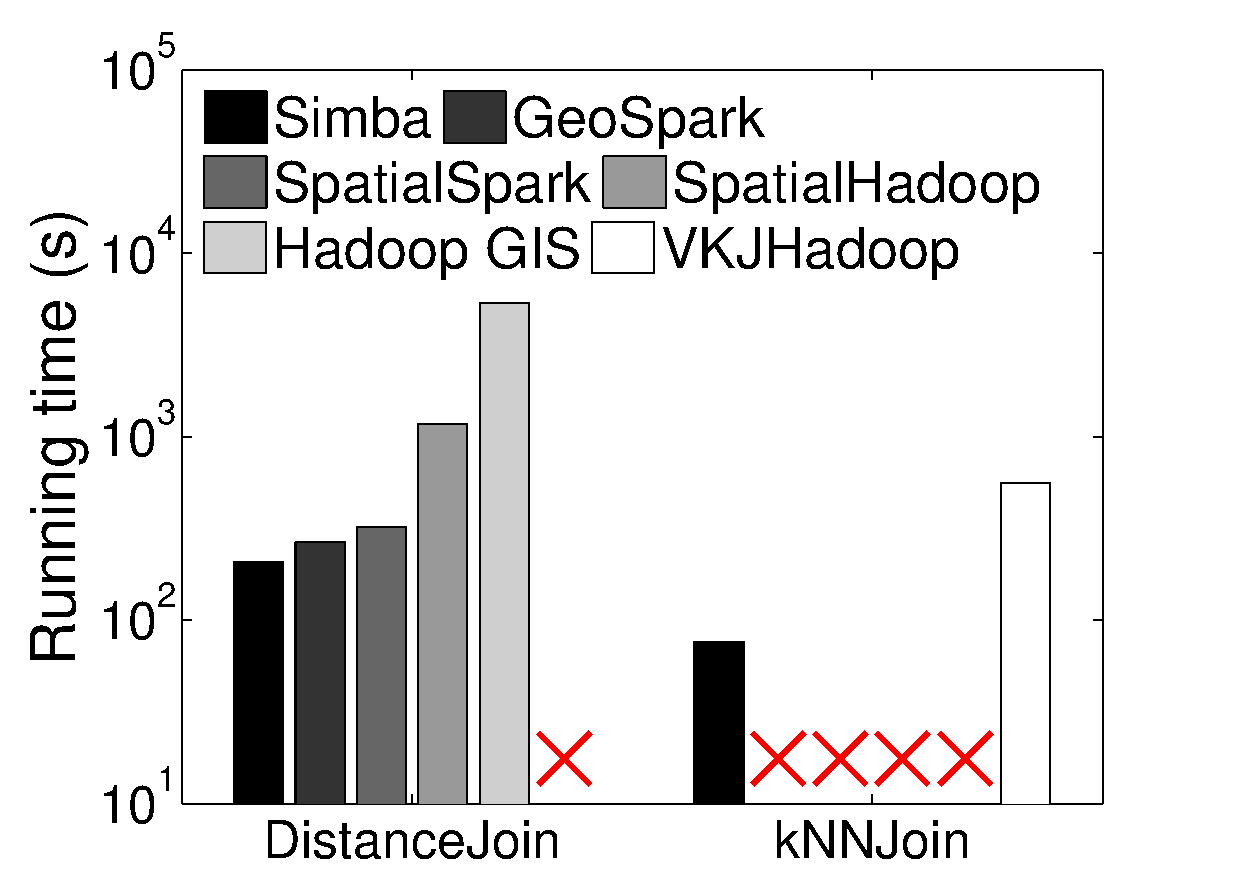
\includegraphics[width = 1.74in]{figs/exp/osm_join_time}\vspace{-4mm}
%	\caption{Join operations on different systems.}
%	\label{fig:system_join}\vspace{-1mm}
%\end{figure}


Figure \ref{fig:system_single} shows the performance of
single-relation operations using both range and $k$NN queries. As
shown in the figure, \name provides the best system throughput and the
best query latency. Specifically, \name achieves 5-50x better
performance (on both throughput and latency) than all existing spatial
analytics systems. Note that the performance of GeoSpark is even worse
than Hadoop based systems because GeoSpark does not leverage global
indexes in query processing, which can help pruning large numbers
of useless partitions (more than 90\%) before scanning them.

% New Range Results of GeoSpark with local indexes.
% Latency: 740.6194
% Througput: 0.6624490742274187

For join operations (using 3 million records in each table), as shown
in Figure \ref{fig:system_join}, \name runs distance join 1.5x faster
than SpatialSpark and 5x faster than Hadoop GIS. Note that distance join
over point objects is not supported in GeoSpark and SpatialHadoop.
GeoSpark supports spatial join between a point RDD and a circle RDD.
Thus, we map each element of $R$ from a point $r$ to a circle object
which centers at $r$ with a radius $\tau$ to a new table $RC(\tau)$.
Immediately, $R \Join_{\tau} S = RC(\tau)\Join_{\textrm{contains}} S$
which is a spatial join. As to SpatialHadoop, it only supports spatial
join over geometric objects, we use $RC(\tau/2)\Join_{\textrm{intersects}} SC(\tau/2)$
to calculate the original distance join.

$k$NN join is not supported by any of these systems. So we compared \name
(using its RKJSpark algorithm) with the Voronoi-based $k$NN join on Hadoop
\cite{vhadoop} (denoted as VKJ-Hadoop), and \name is 7x faster than VKJ-Hadoop.


%       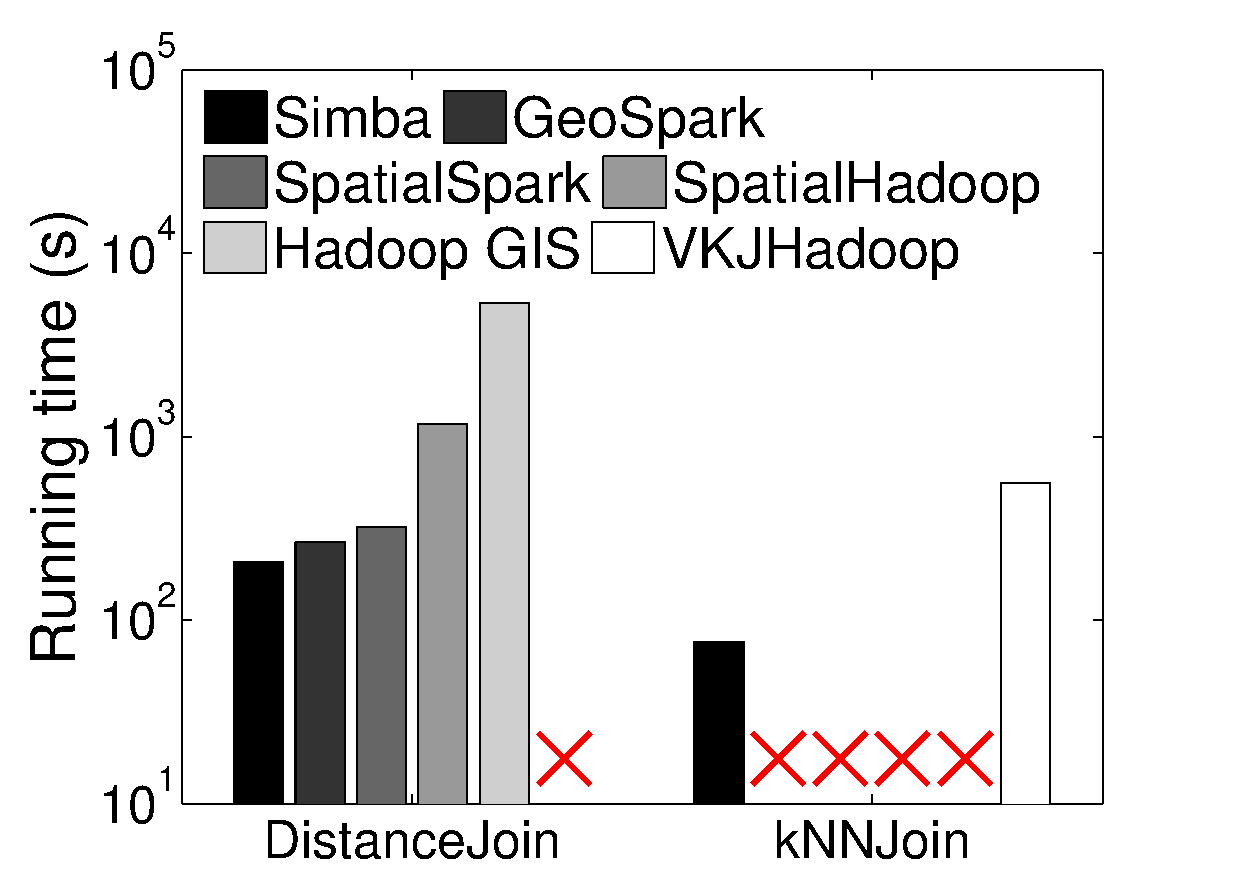
\includegraphics[width = 1.60in]{figs/exp/osm_join_time}\vspace{-2mm}
%       \caption{Join operations on different systems.}
%       \label{fig:system_join}

\begin{wrapfigure}{l}{0.15\textwidth}
 \centering
 \vspace*{-0.2cm}
  \hspace*{-0.3cm}
  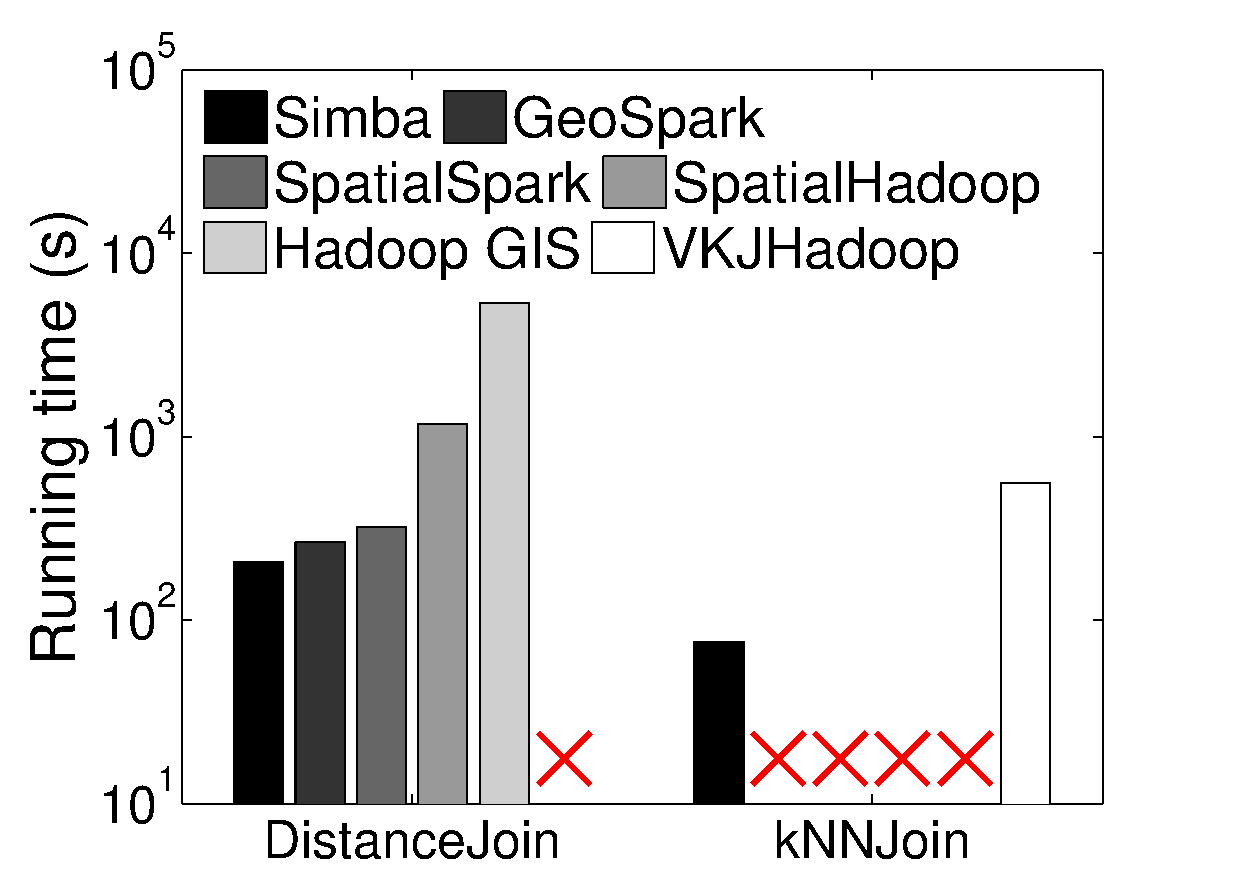
\includegraphics[width=1.5in]{figs/exp/osm_join_time}
  \vspace*{-0.80cm}
  \caption{\label{fig:system_join}Joins in different systems.}\vspace{-2mm}
\end{wrapfigure}
\name is more efficient than SpatialSpark \cite{spatialspark} and
GeoSpark\cite{geospark}, since they are {\em only a library runs on
top of and outside Spark without a query engine}. In contrast, \name
is full-fledged spatial query engine that extends the core of Spark SQL.
Compared to Hadoop based systems like SpatialHadoop \cite{spatialhadoop}
and Hadoop GIS \cite{hadoopgis}, \name extends the engine of Spark SQL
to support spatial operations natively with a sophisticated, RDBMS-like
query engine, and uses Spark for in-memory computation, hence, is much
more efficient. For example, \name provides 51x lower latency and 45x
higher throughput than SpatialHadoop for $k$NN queries. That said,
Hadoop-based systems will be useful when data is so large that they
cannot fit into the cluster's memory space.

Lastly, note that \name is also much more user-friendly with the
native support on both SQL and DataFrame query interfaces over {\em
both spatial and non-spatial operations}, which are {\em not}
supported by any of the other systems (SpatialHadoop supports a
SQL-like query language Pigeon, an extension of Pig). That said, in
the following, we focus on comparing \name with Spark SQL, where we
support various spatial operations in Spark SQL by directly expressing
a spatial operation in its standard SQL syntax if it is possible, or
using UDFs in SQL when this is not possible.

\subsection{Comparison against Spark SQL}

\begin{figure}[!t]
	\centering
	\subfigure[Effect of data size.]{
		\label{fig:osm_rect_datasize}
		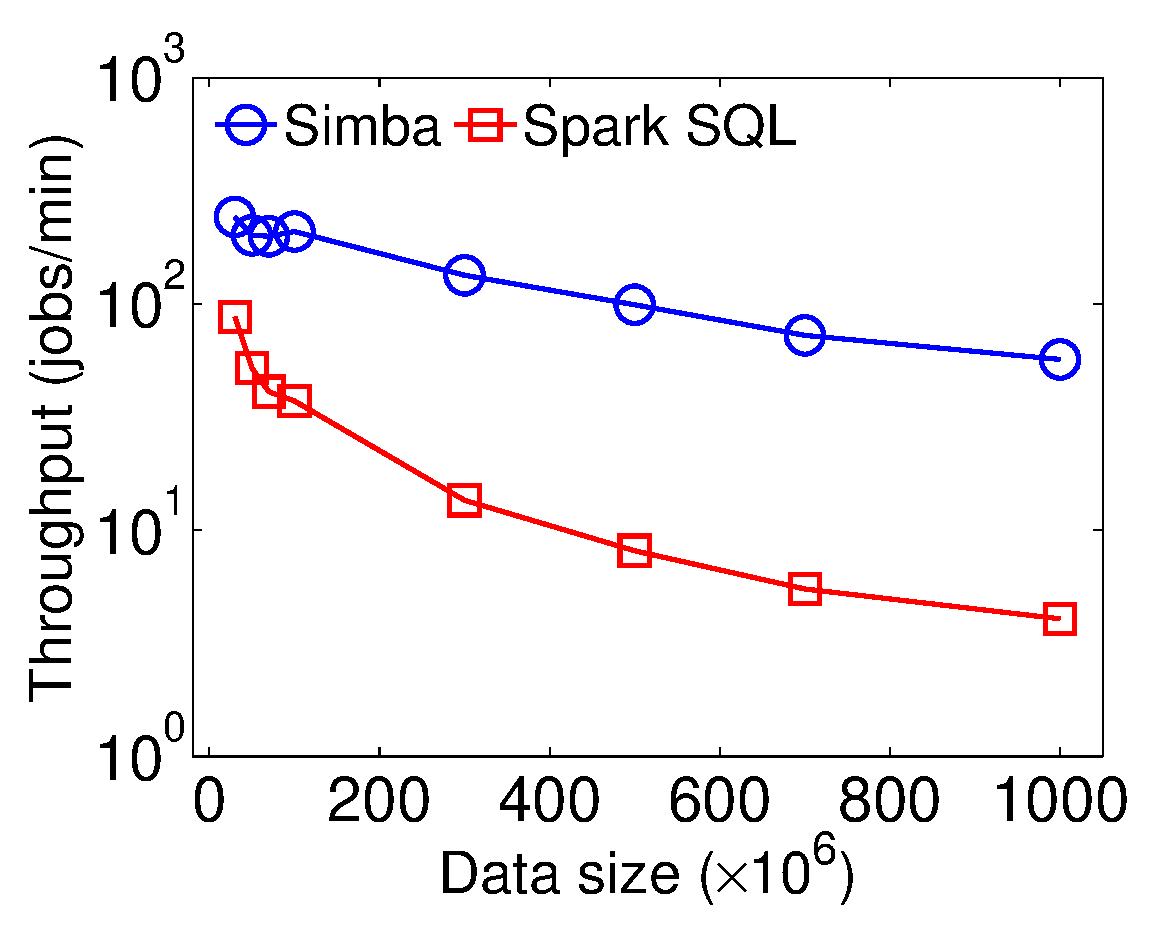
\includegraphics[width=1.55in]{figs/exp/osm_rect_datasize_throughput}
		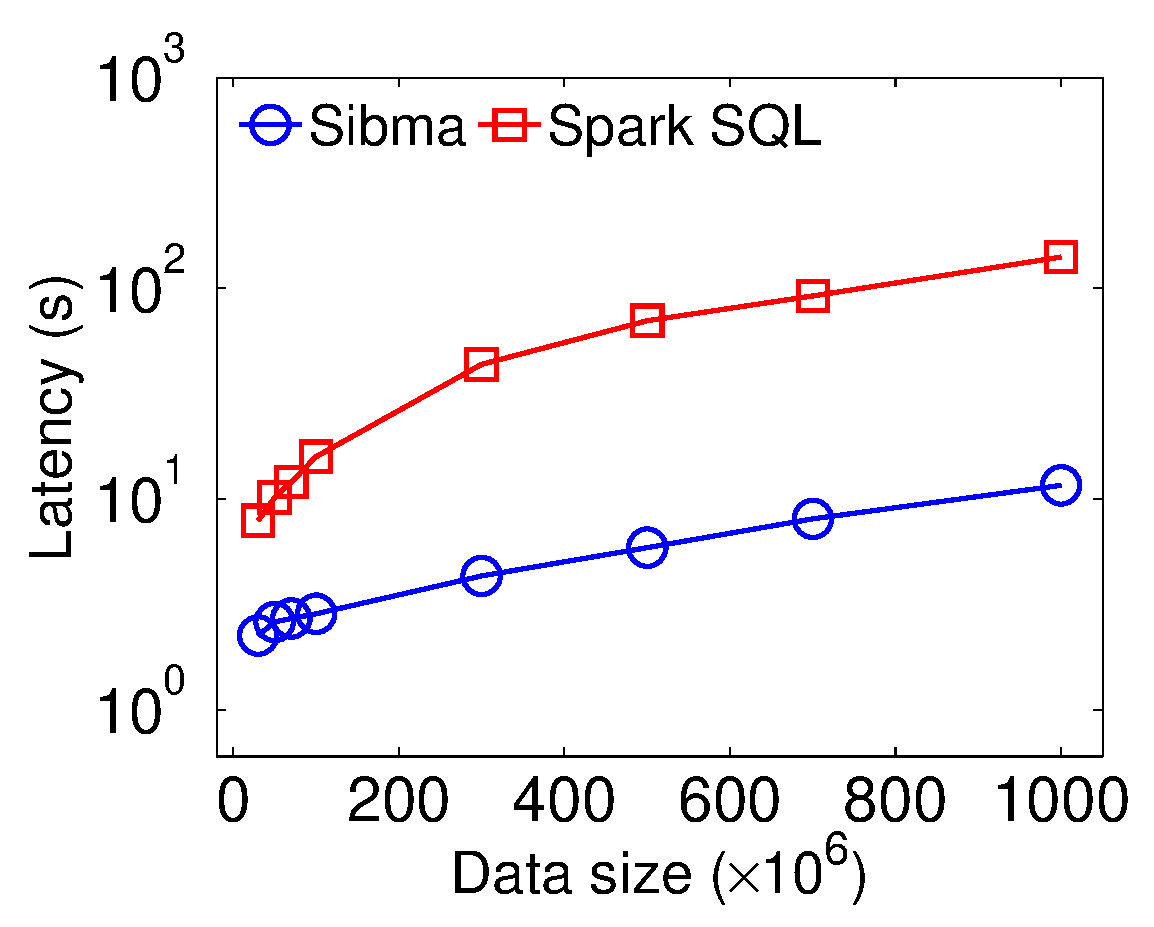
\includegraphics[width=1.55in]{figs/exp/osm_rect_datasize_latency}
	} \vspace{5mm}

	\subfigure[Effect of query area size (percentage of total area).]{
		\label{fig:osm_rect_rate}
		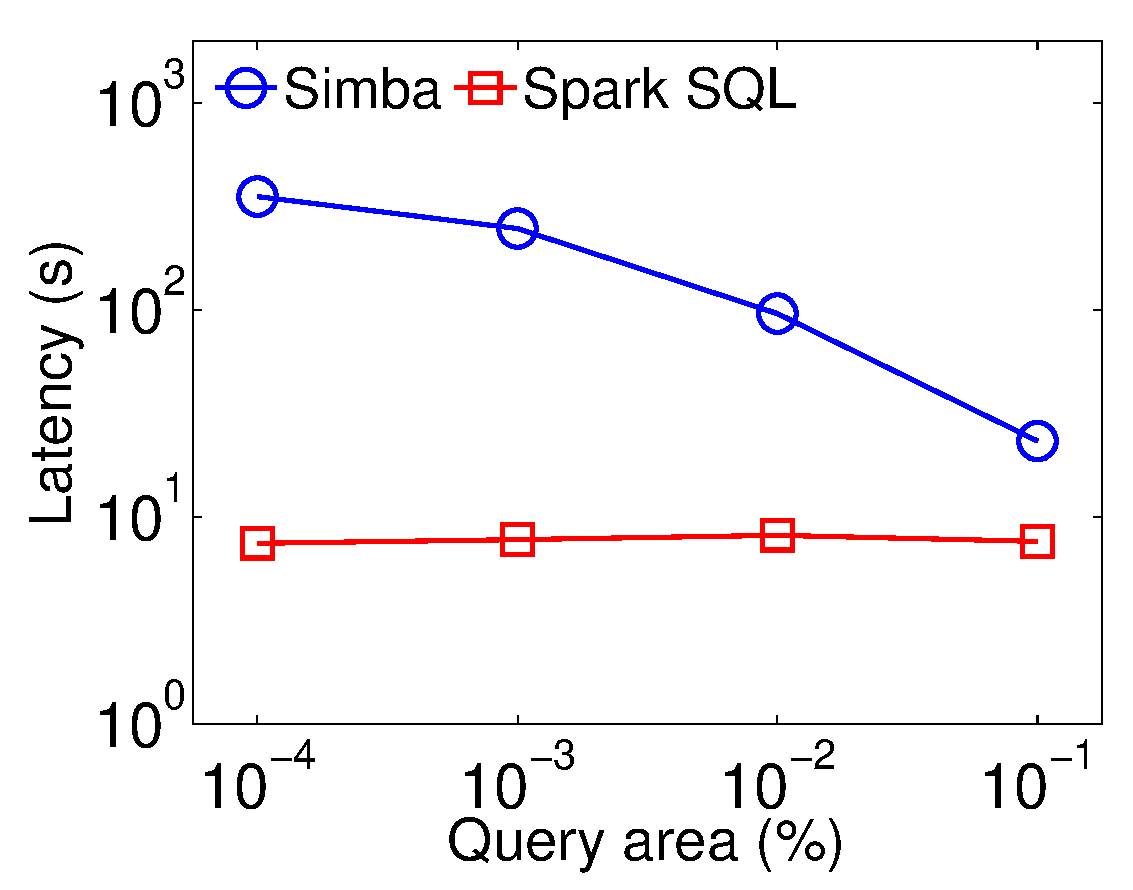
\includegraphics[width=1.55in]{figs/exp/osm_rect_rate_throughput}
		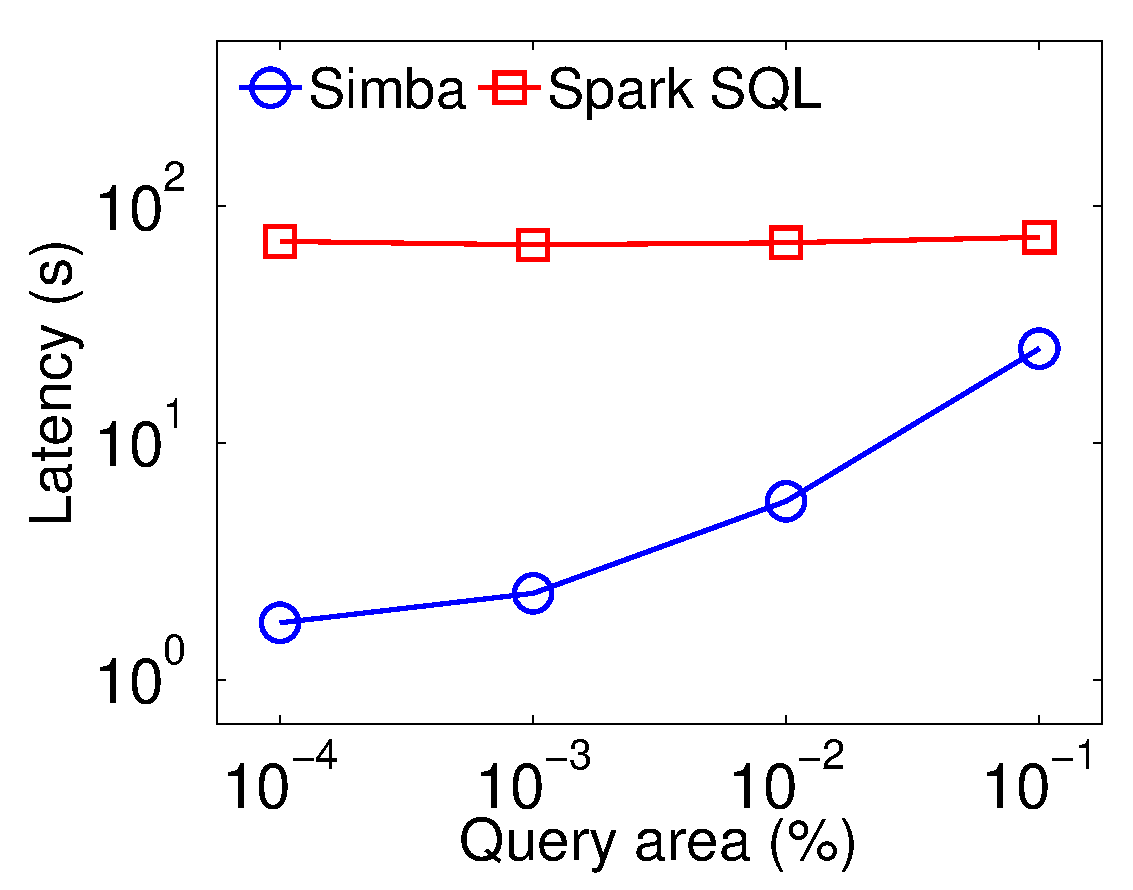
\includegraphics[width=1.55in]{figs/exp/osm_rect_rate_latency}
	} %\vspace{5mm}
	% \subfigure[Effect of partition size (number of records per partition).]{
	% 	\label{fig:osm_rect_partsize}
	% 	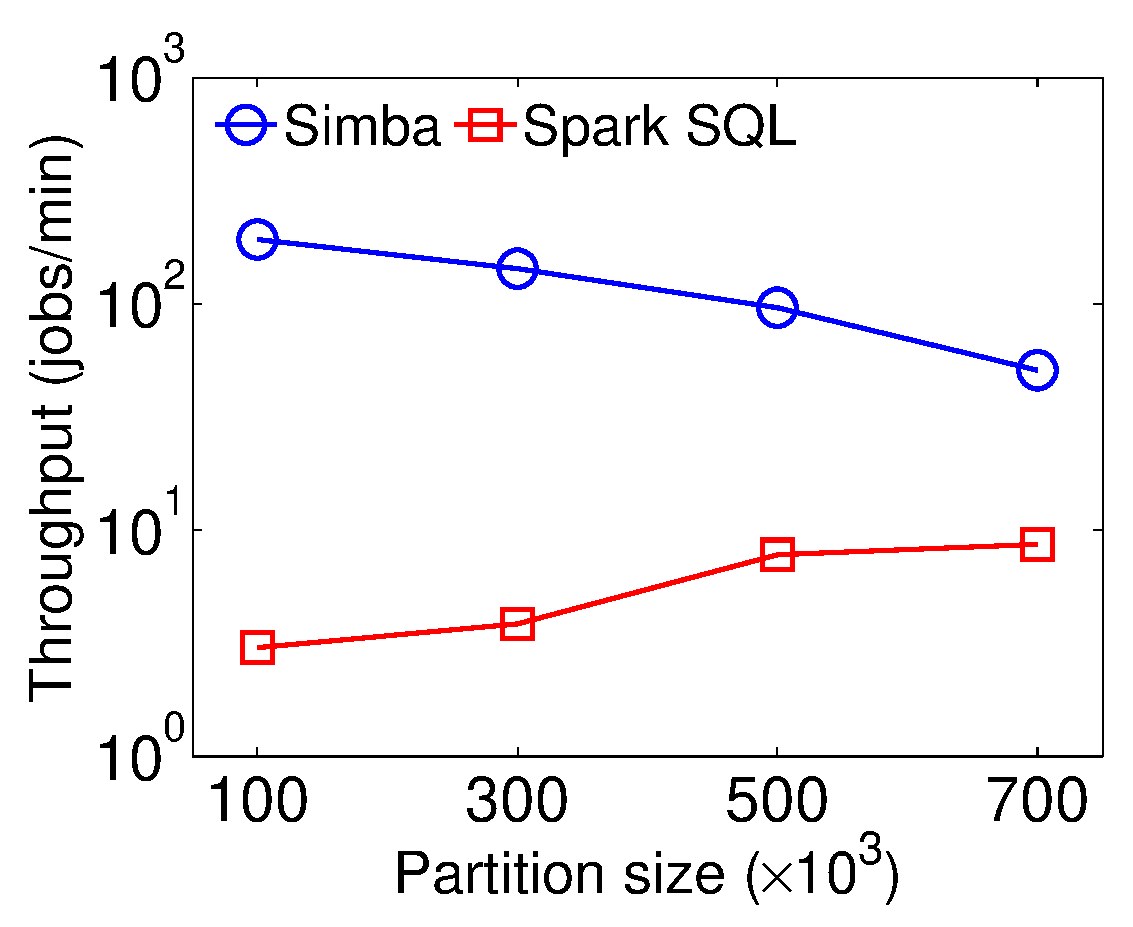
\includegraphics[width=1.55in]{figs/exp/osm_rect_partsize_throughput}
	% 	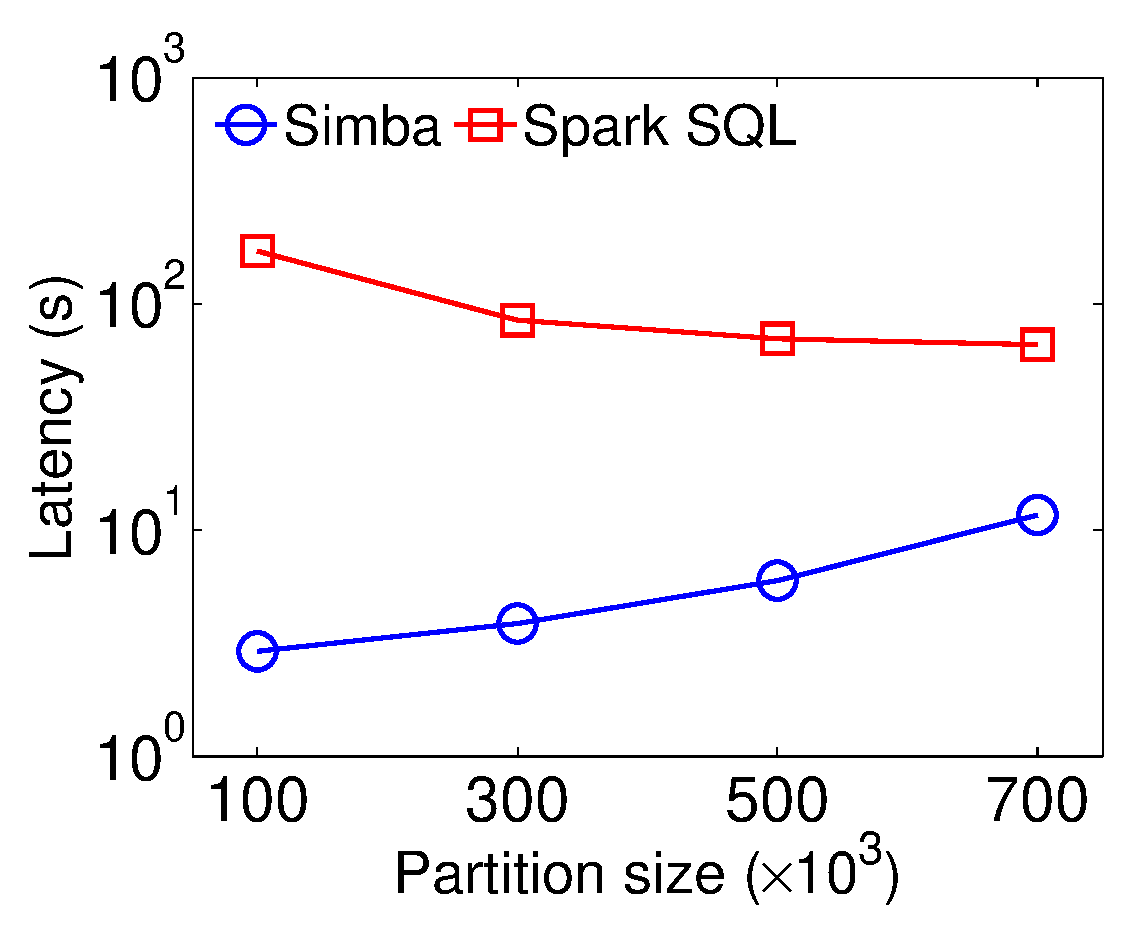
\includegraphics[width=1.55in]{figs/exp/osm_rect_partsize_latency}
	% }
	\caption{Range query performance on OSM.}
	\label{fig:range}\vspace{-5mm}
\end{figure}

\Paragraph{Range queries.}
Figure \ref{fig:range} shows the performance of range queries in both
engines using the OSM data set. Queries are centered at random points
sampled from the input data. As a result, the query workload fits well
with the distribution of the data, where dense areas will be queried
with higher probabilities.

Figure \ref{fig:osm_rect_datasize} shows that \name outperforms Spark
SQL by about one order of magnitude on both query throughput and query
latency.  The performance of both \name and Spark SQL drops when data
size increases while that of \name drops much slower, which implies
\name has much better scalability. This is because of spatial index
and spatial-aware optimization in \name: larger data size does lead to
more partitions to process and larger output size, but it also implies
potentially more pruning power from its indexes and optimizer. In
contrast, Spark SQL has to scan the whole table regardless.

Figure \ref{fig:osm_rect_rate} shows how throughput and latency are
influenced by the size of the query area. As the query area enlarges,
performance of \name becomes closer to that of Spark SQL. The reason
for this is the result size becomes very large and there is less
optimization opportunities for \name's query optimizer. Spark SQL's
query performance is {\em hardly} affected by the size of the query
area, since it has to scan the whole table regardless.

\Paragraph{$k$NN queries.}
Figure \ref{fig:knn} shows the performance of $k$NN queries on Spark
SQL and \name, using the OSM data set, where query points are randomly
sampled from the input data.
Figure \ref{fig:osm_knn_datasize} measures system throughput and query
latency when increasing the data size from 30 million to 1 billion
records. \name achieves one to two orders of magnitude better
performance on both metrics. Spark SQL's performance drops
significantly as data becomes larger, since it requires scanning the
whole table for a $k$NN query, while \name's performance is almost not
affected by the data increase since regardless of the data size, \name
is able to narrow down quickly to just a few RDD partitions that may
contain the $k$NNs.

Next, using the default data size which is 500 million records, we
study the impact of $k$. As $k$ varies from $1$ to $50$ in Figure
\ref{fig:osm_knn_k}, \name maintains a speedup of two orders of
magnitude. Both \name and Spark SQL's performance are not really
affected by $k$: Spark SQL needs to scan the data regardless of $k$
values; whereas \name's performance will not change much when the
change in $k$ is much smaller compared to the partition size.


\begin{figure}[!t]
	\centering
	\subfigure[Effect of data size.]{
		\label{fig:osm_knn_datasize}
		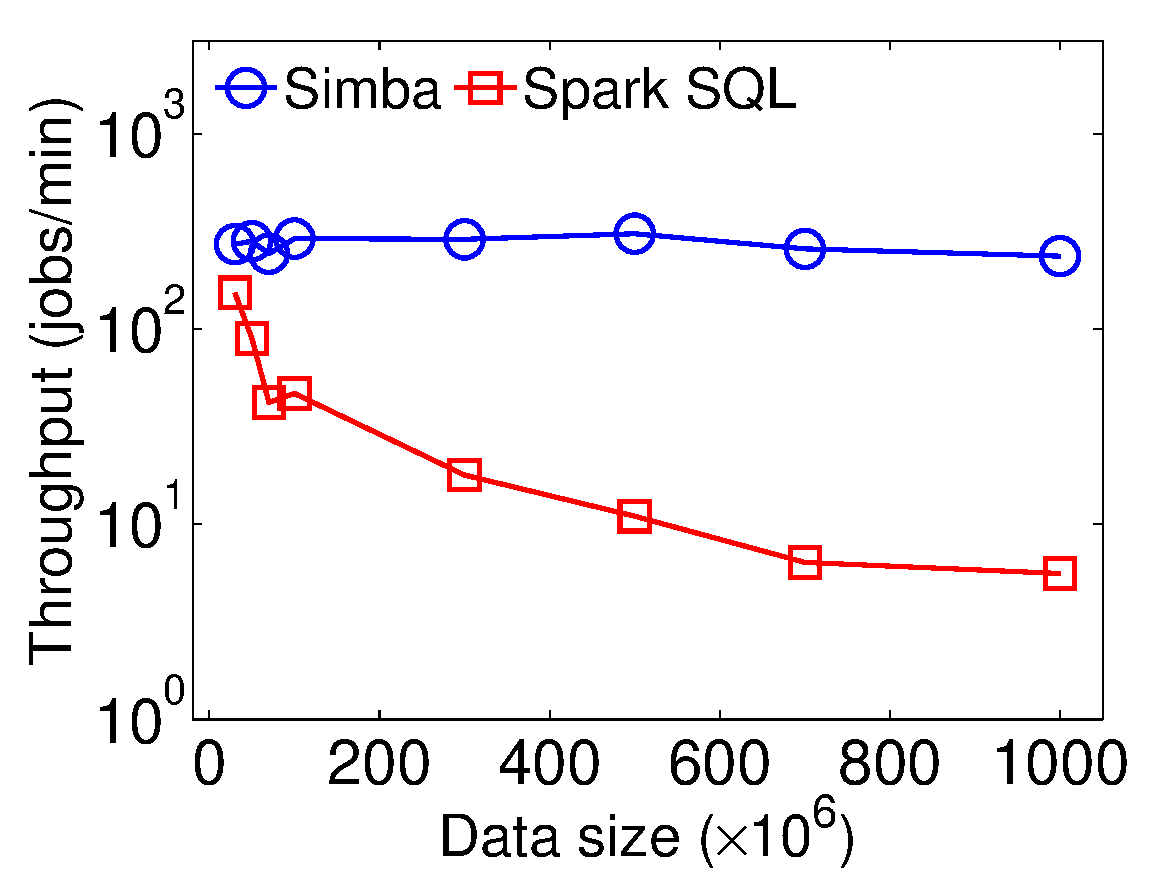
\includegraphics[width=1.55in]{figs/exp/osm_knn_datasize_throughput}
		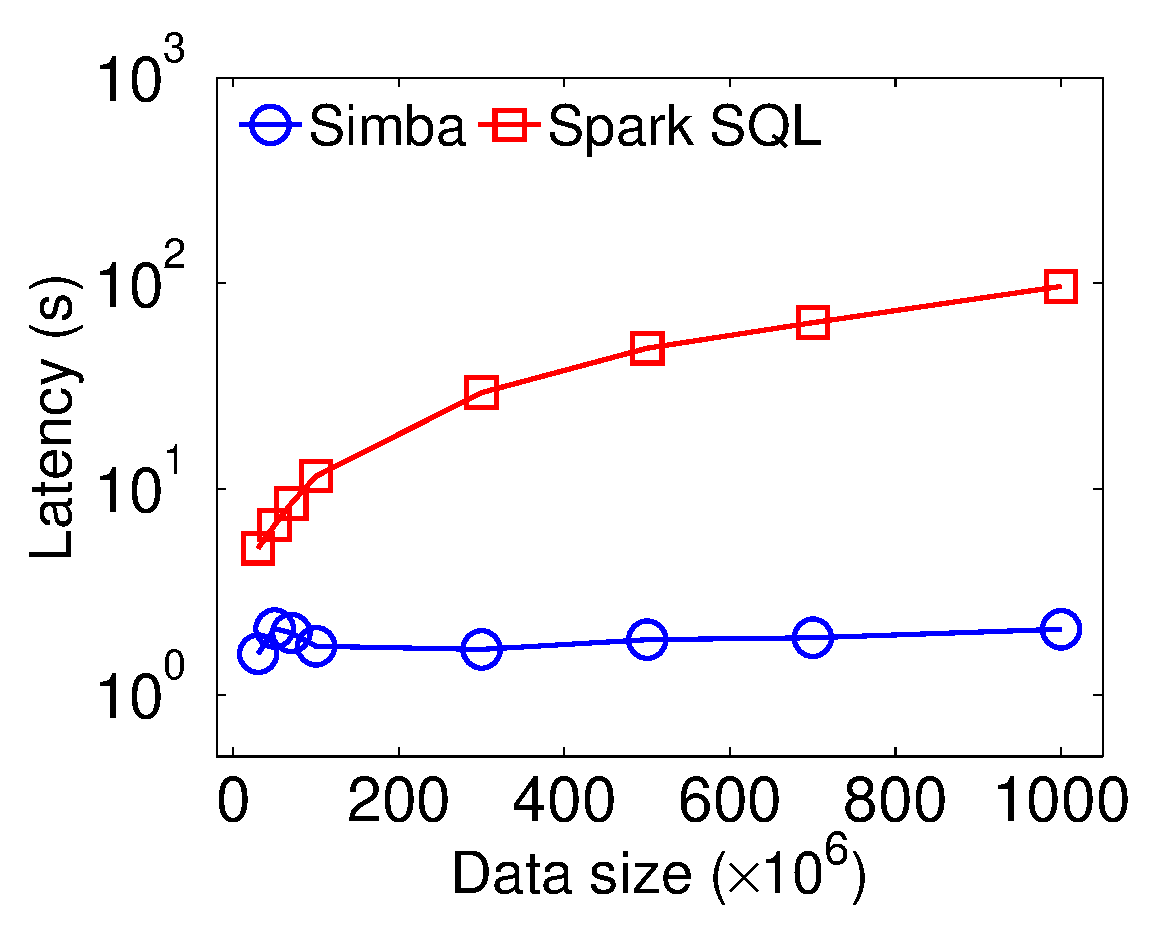
\includegraphics[width=1.55in]{figs/exp/osm_knn_datasize_latency}
	} \vspace{4mm}

	\subfigure[Effect of $k$.]{
		\label{fig:osm_knn_k}
		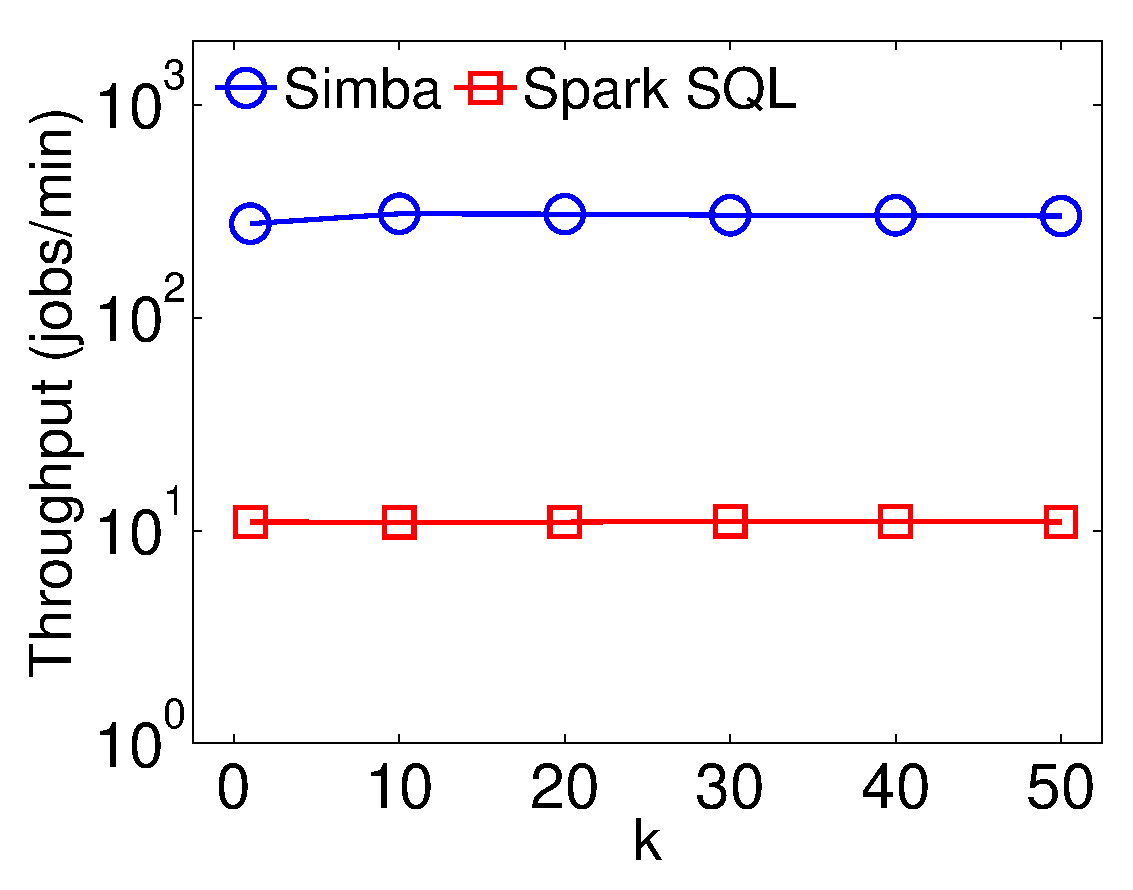
\includegraphics[width=1.55in]{figs/exp/osm_knn_k_throughput}
		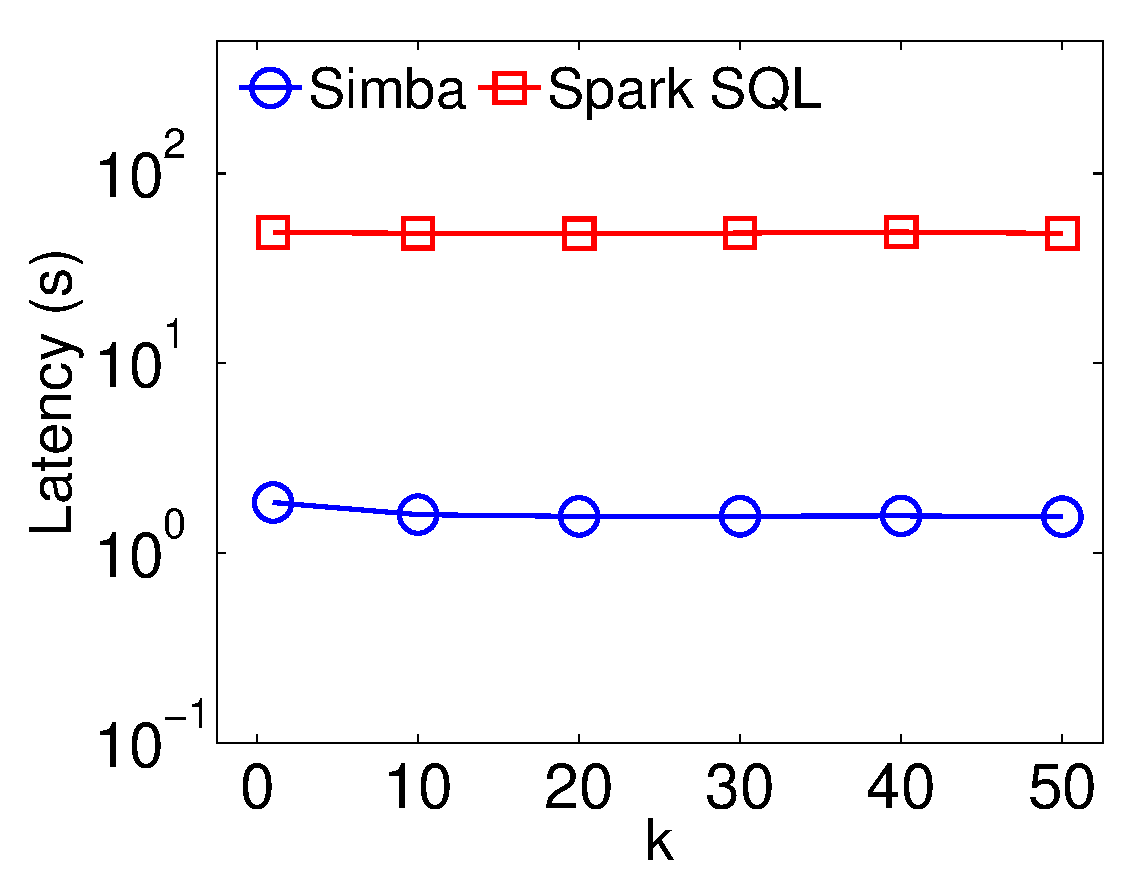
\includegraphics[width=1.55in]{figs/exp/osm_knn_k_latency}
	} % \vspace{4mm}

	% \subfigure[Effect of partition size (number of records per partition).]{
	% 	\label{fig:osm_knn_partsize}
	% 	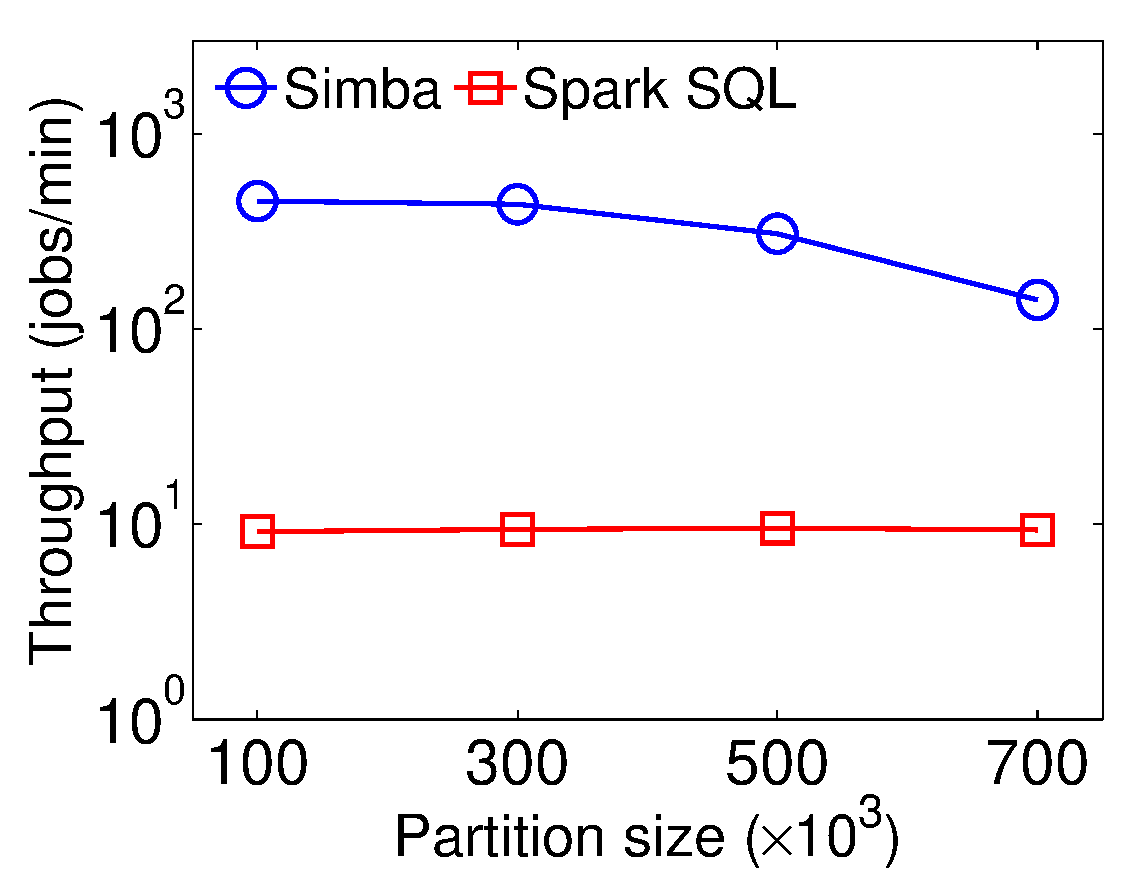
\includegraphics[width=1.55in]{figs/exp/osm_knn_partsize_throughput}
	% 	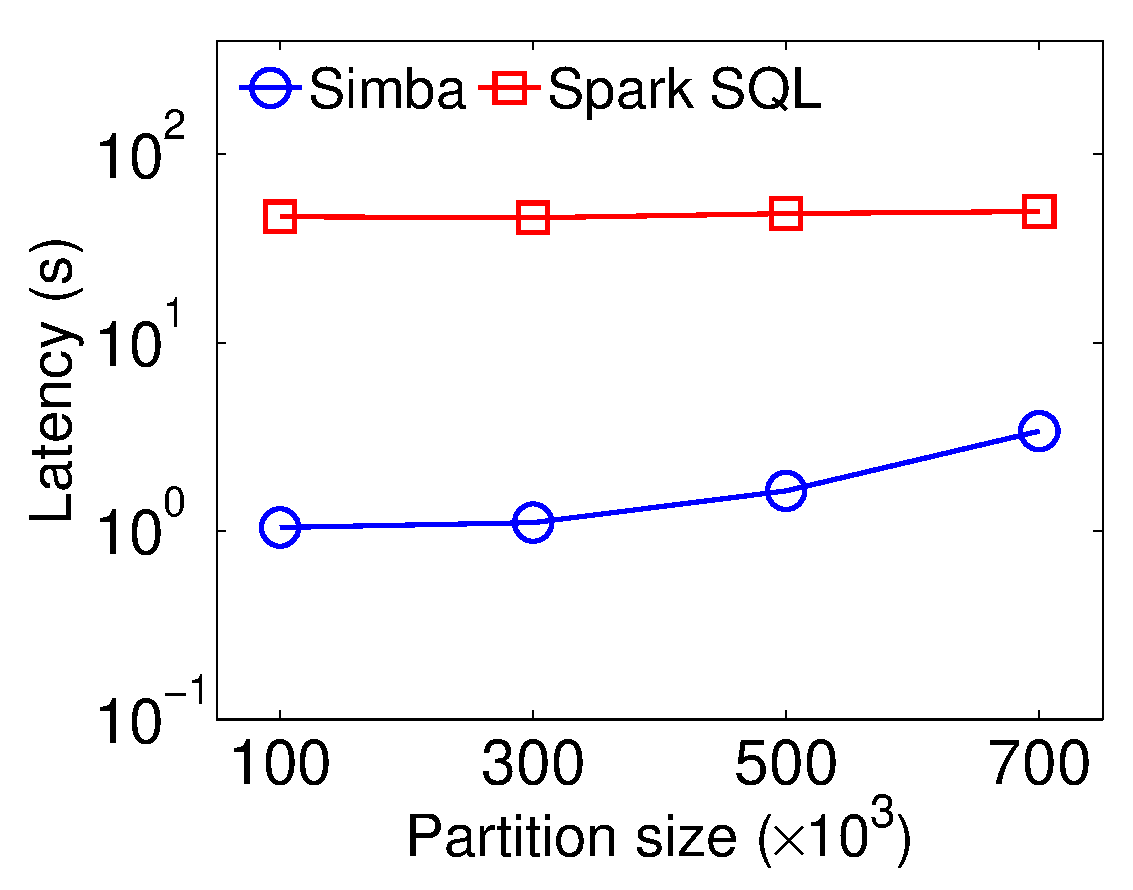
\includegraphics[width=1.55in]{figs/exp/osm_knn_partsize_latency}
	% }\vspace{0mm}
	\caption{$k$NN query performance on OSM.}\vspace{-4mm}
	\label{fig:knn}
\end{figure}



\Paragraph{Distance join.}
Figure \ref{fig:disj} shows the results of the distance join
experiments, using two tables sampled from OSM (each is 3 million
records). We tried expressing and running a distance join as an
$\theta$-join in Spark SQL (an example was shown in Section
\ref{sub:disjoin}). However, {\em it did not finish in 10 hours when
  joining two tables of only 1 million records, and crashed, due to
  the expensive cartesian product it has to perform}.


\begin{figure}[!t]
	\subfigure[Effect of data size.]{
		\label{fig:osm_disj_datasize}
		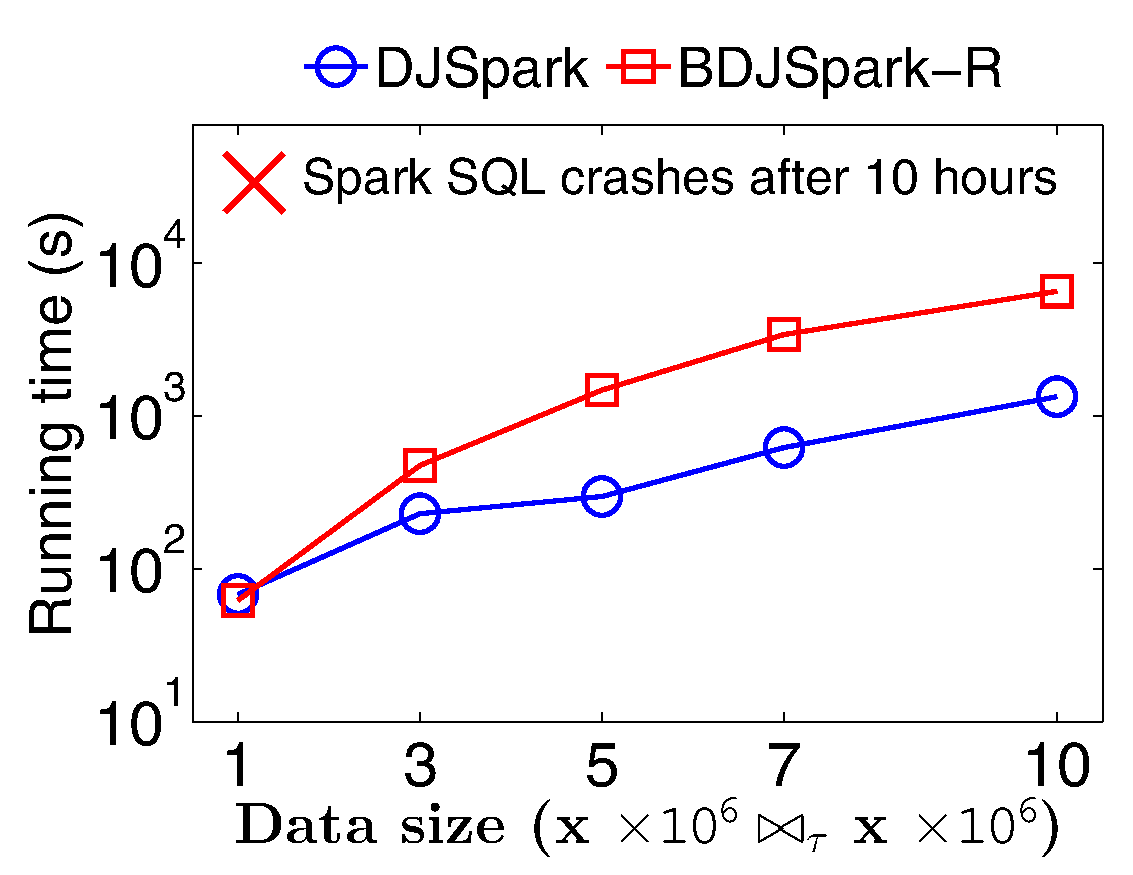
\includegraphics[width=1.55in]{figs/exp/osm_disj_datasize}
	} %\vspace{6mm}
	\subfigure[Effect of $\tau$.]{
		\label{fig:osm_disj_rate}
		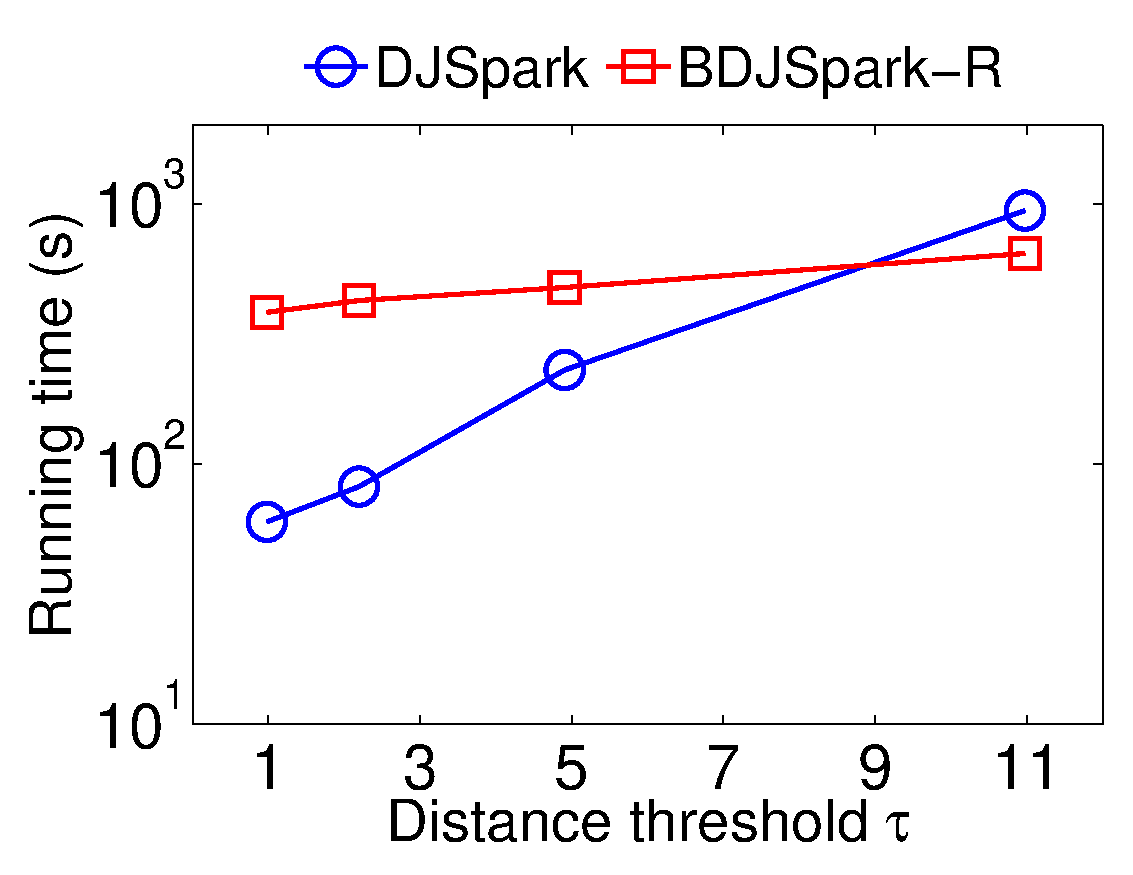
\includegraphics[width=1.55in]{figs/exp/osm_disj_rate}
	} %\vspace{6mm}
	%\centering
	%\subfigure[Effect of expected partition size]{
	%	\label{fig:osm_disj_partsize}
	%	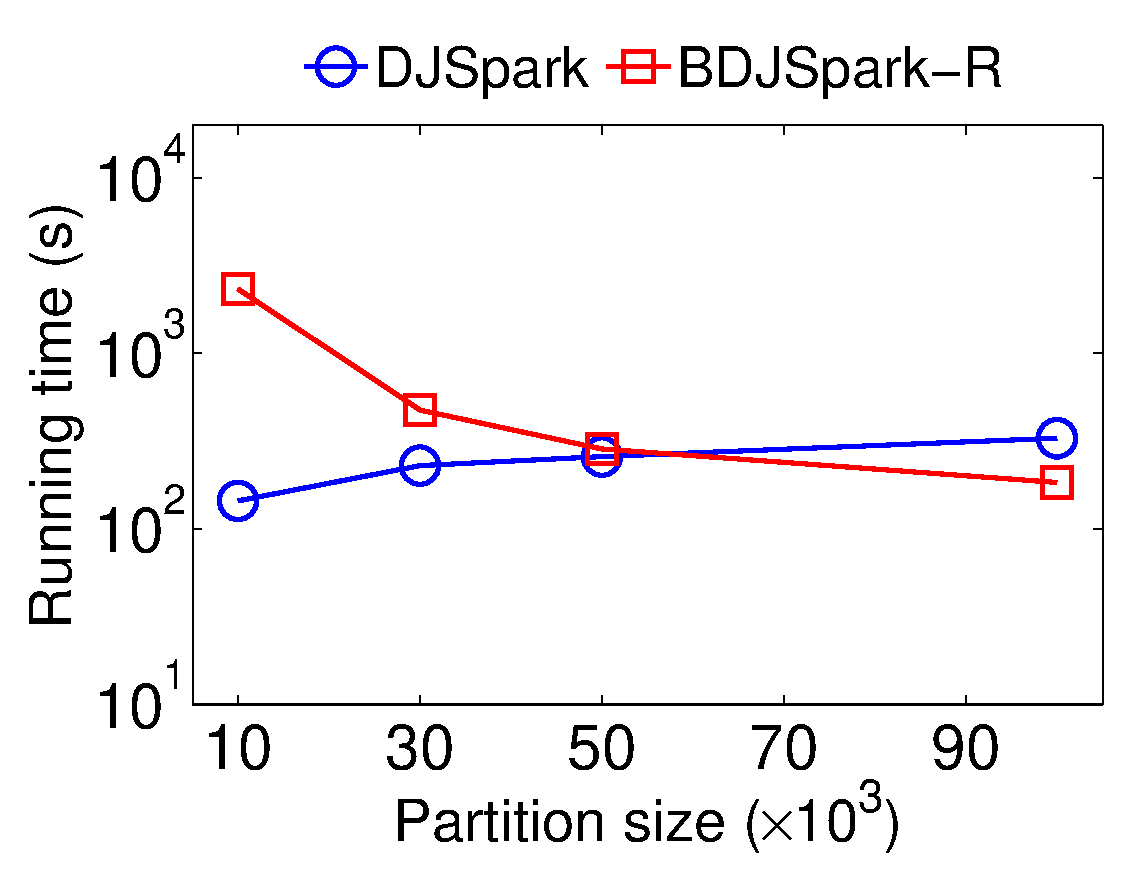
\includegraphics[width=1.74in]{figs/exp/osm_disj_partsize}
  %} \vspace{-6mm}
	\caption{Distance join performance on OSM.}
	\label{fig:disj}\vspace{-3mm}
\end{figure}


\begin{figure}[!t]
	\subfigure[Effect of data size.]{
		\label{fig:osm_knnj_datasize}
		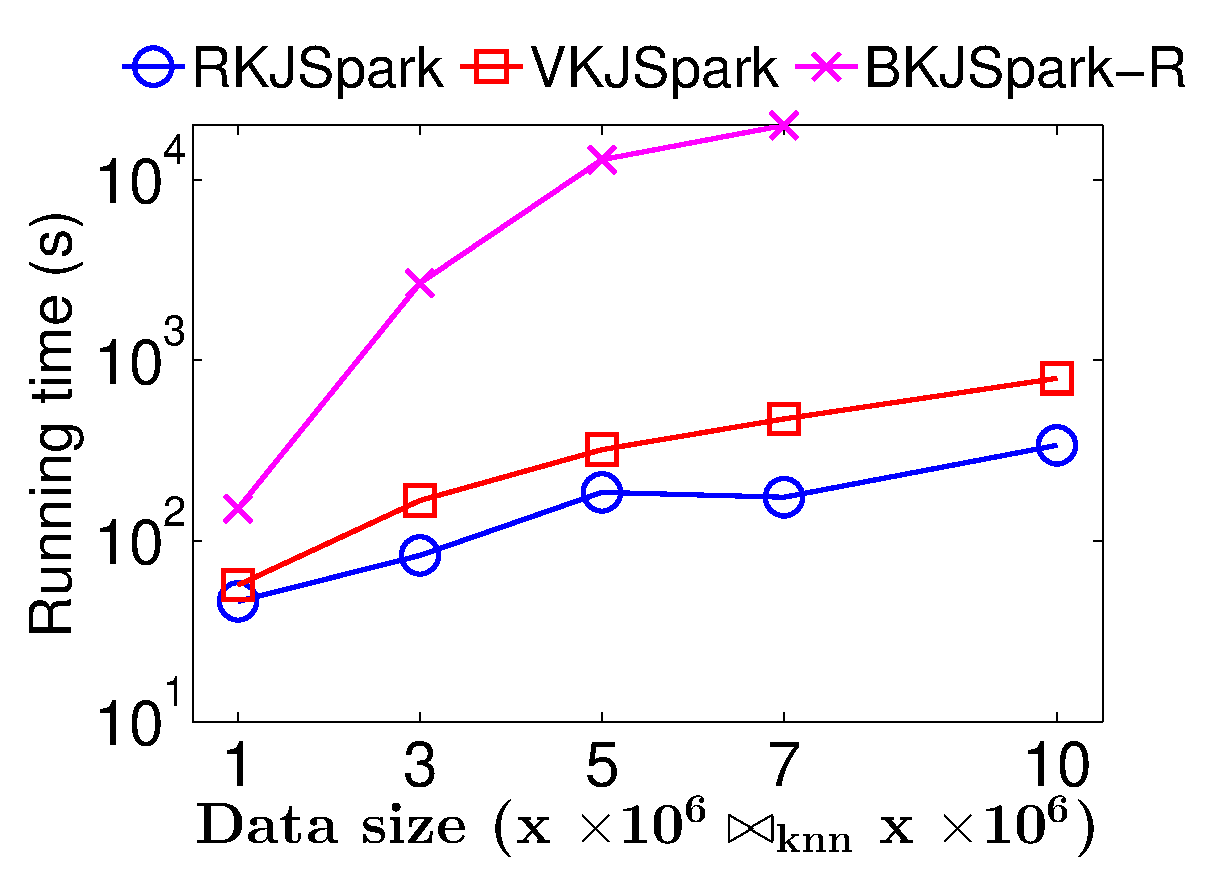
\includegraphics[width = 1.55in]{figs/exp/osm_knnj_datasize}
	} %\vspace{6mm}
	\subfigure[Effect of $k$.]{
		\label{fig:osm_knnj_k}
		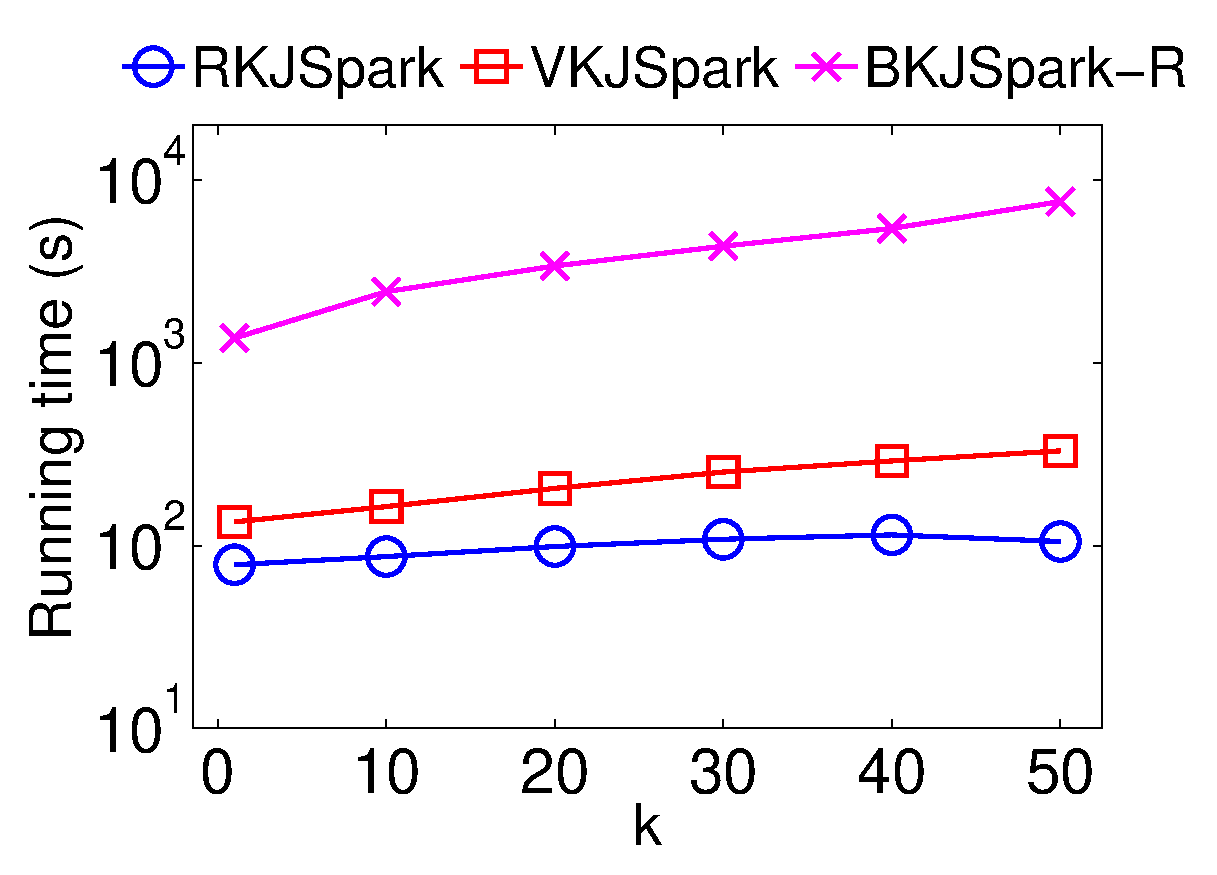
\includegraphics[width = 1.55in]{figs/exp/osm_knnj_k}
	} %\vspace{6mm}
	%\centering
	%\subfigure[Effect of expected partition size]{
	%	\label{fig:osm_knnj_partsize}
	%	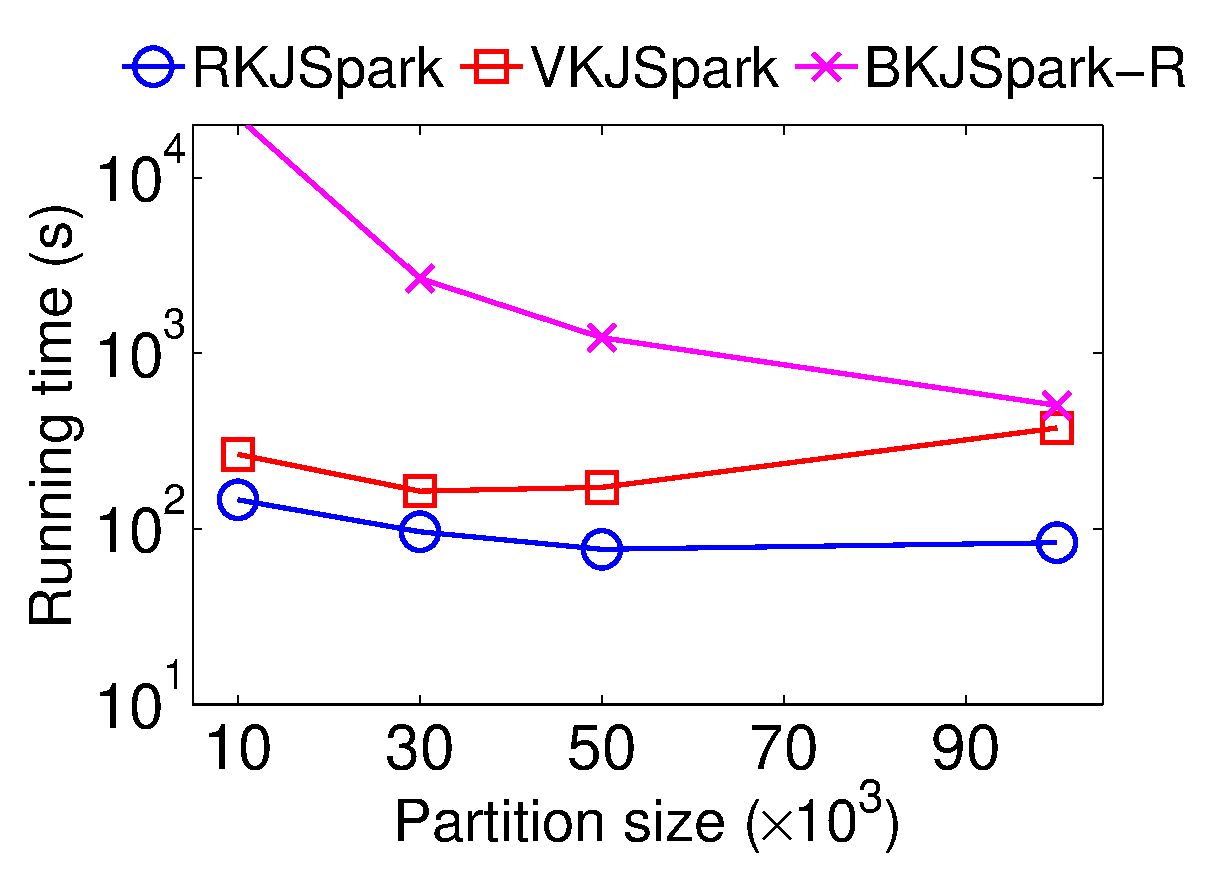
\includegraphics[width=1.74in]{figs/exp/osm_knnj_partsize}
	%} \vspace{-5mm}
	\caption{$k$NN join performance on OSM.}
	\label{fig:knnj}\vspace{-4mm}
\end{figure}


For \name, we compared the algorithm DJSpark as introduced in Section
\ref{sub:disjoin} and a nested loop join approach using R-trees as
local indexes, termed as BDJSpark-R (a simple variation of BKJSpark-R
discussed in Section \ref{sub:knnjoin}; replacing each local $k$NN
join with a local distance join).

% \dong{We did not introduce the nested-loop version (with R-Tree) and
%   the hash join version for distance joins in this paper. I
%   temporarily term the nested-loop version as BDJSpark-R, and the
%   hash-join version as HDJSpark.}

Naturally, the cost of both algorithms increase with larger input size
(Figure \ref{fig:osm_disj_datasize}) and larger distance threshold
(Figure\ref{fig:osm_disj_rate}). Nevertheless, DJSpark is always more
efficient than the baseline method BDJSpark-R, unless the threshold
grows to a relatively large value (say $x=11$ in this case; roughly
1\% of the space). % (\feifei{specify this distance value
  % and the average points retrieved}).

%In Figure \ref{fig:osm_disj_partsize}, as expected partition size grows,
%running time of DJSpark and HDJSpark increases slightly as the pruning
%power of the global join phase reduces when partition granularity is
%decreasing. In contrast, BDJSpark-R becomes faster since fewer local
%join tasks are required for processing.

\Paragraph{$k$NN join.}
It is {\em impossible to express $k$NN join in Spark SQL}, unless
using $N$ union statements where $N$ is the number of records in the
first input table, which is clearly not a practical solution for large
tables. Hence, we focused on comparing different $k$NN join algorithms
in \name.

Figure \ref{fig:knnj} shows the performance over OSM data (default is
$3$ million records in each input table and $k=10$). clearly, RKJSpark
shows the best performance and best scalability (wrt both data size
and $k$). As an example, for a $k$NN join between two 5 million
records tables, RKJSpark join is 3x faster than VKJSpark and 70x
faster than BKJSpark-R. Note that BKJSpark-R strictly dominates
BKJSpark-N, hence, the later is omitted.

% Figure \ref{fig:osm_knnj_k} presents the effect of $k$ on different
% algorithms. With increasing of $k$, running time of BKJSpark-R and
% VKJSpark join grows faster than that of RKJSpark. This is mainly
% because RKJSpark leverages the power of local indexes.

%In Figure \ref{fig:osm_knnj_partsize}, as expected partition size
%increases, BKJSpark-R and RKJSpark become faster since fewer local
%join tasks are required for processing.  VKJSpark runs slightly slower
%when expected partition size increases as the power of its pruning
%bounds weakens with the decreasing on pivot number.

\begin{figure}[t!]
	\centering
	% \subfigure[Synthetic]{
	% 	\label{fig:synthetic_rect_dimension}
	% 	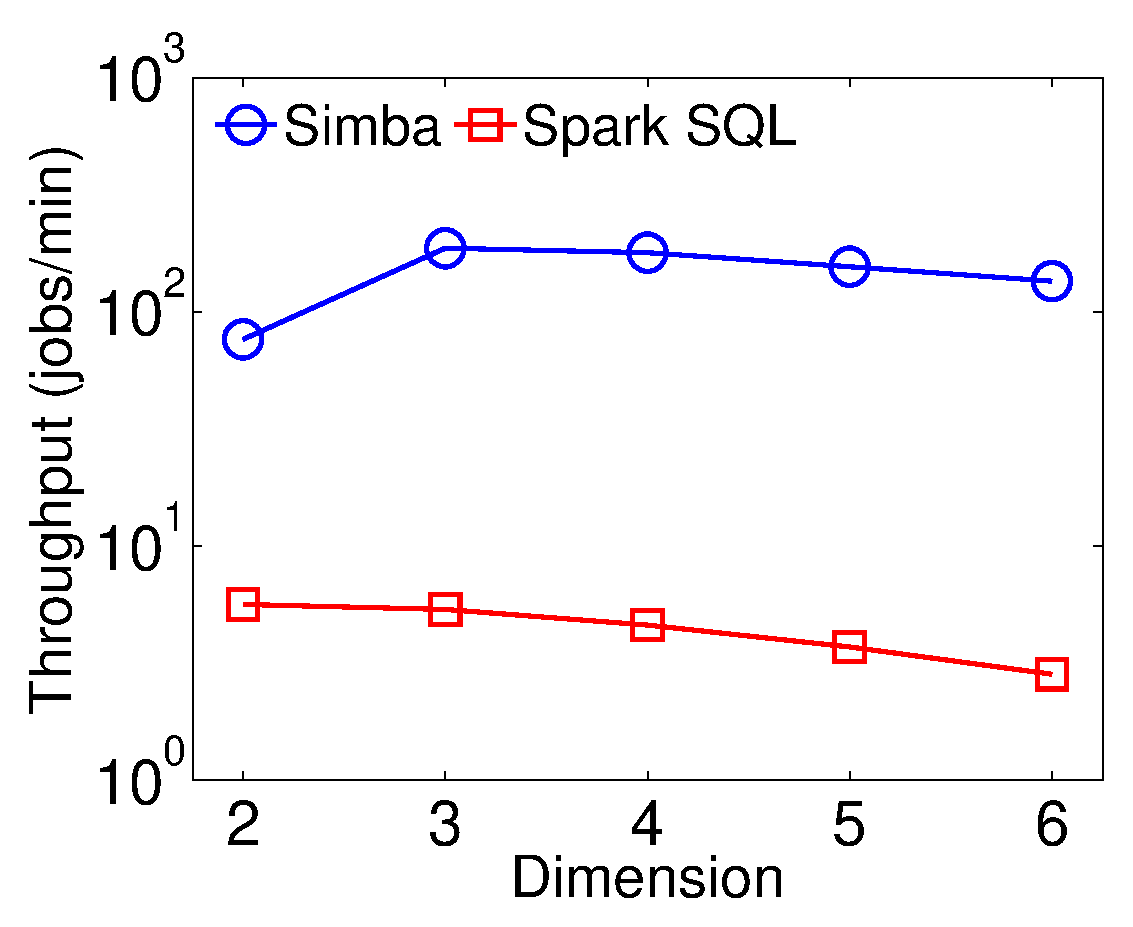
\includegraphics[width=1.55in]{figs/exp/gaussian700m_rect_dimension_throughput}
	% 	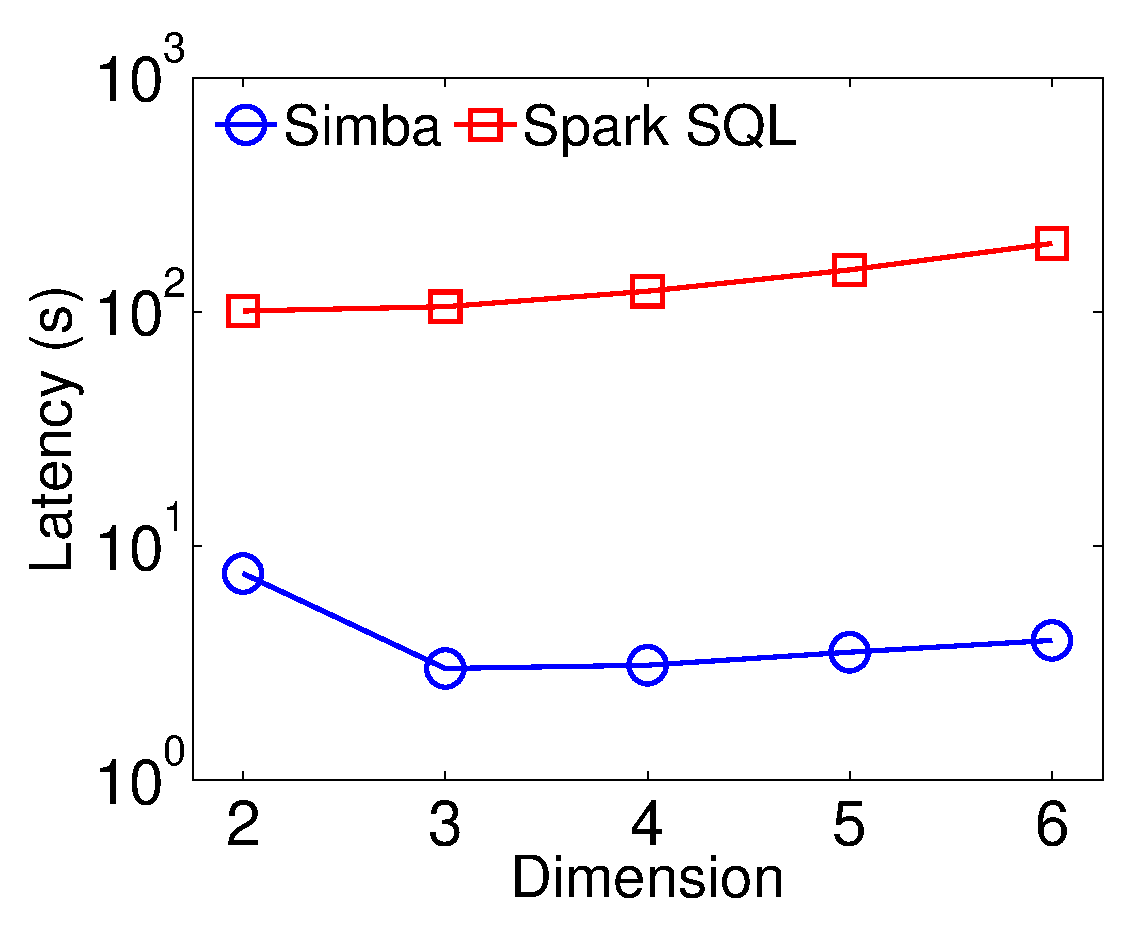
\includegraphics[width=1.55in]{figs/exp/gaussian700m_rect_dimension_latency}
	% }
	
	\subfigure[Throughput] {
		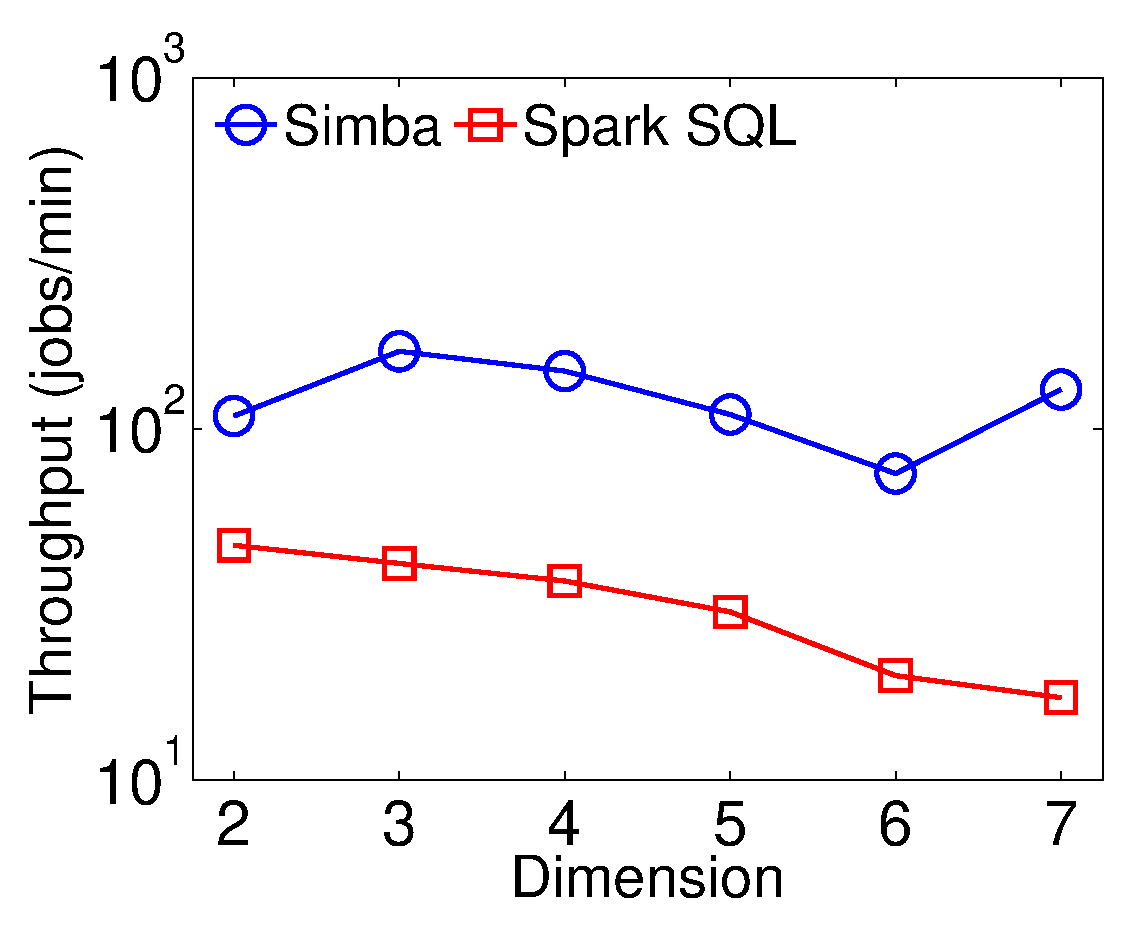
\includegraphics[width=1.55in]{figs/exp/gdelt_rect_dimension_throughput}
		\label{fig:gdelt_rect_dim_throughput}
	}
	\subfigure[Latency] {
		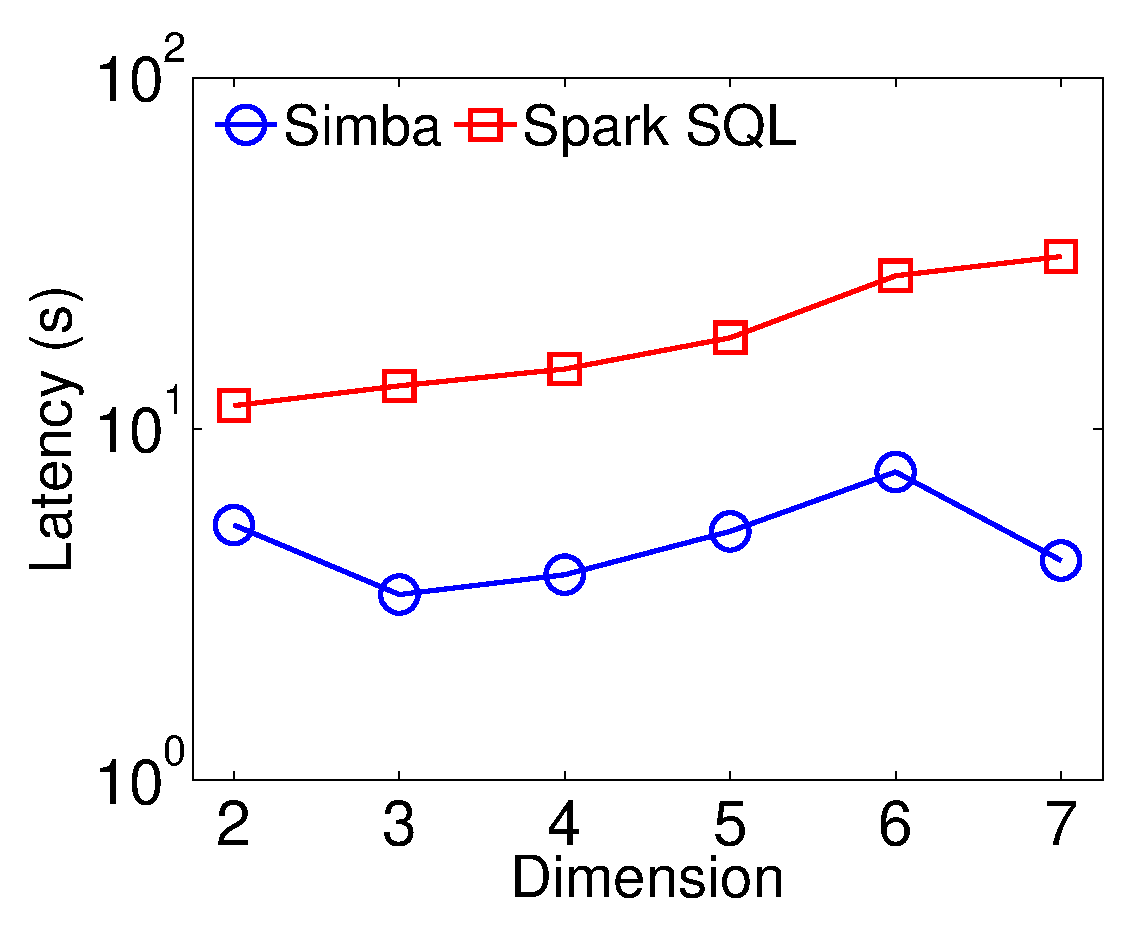
\includegraphics[width=1.55in]{figs/exp/gdelt_rect_dimension_latency}
		\label{fig:gdelt_rect_dim_latency}
	}
	%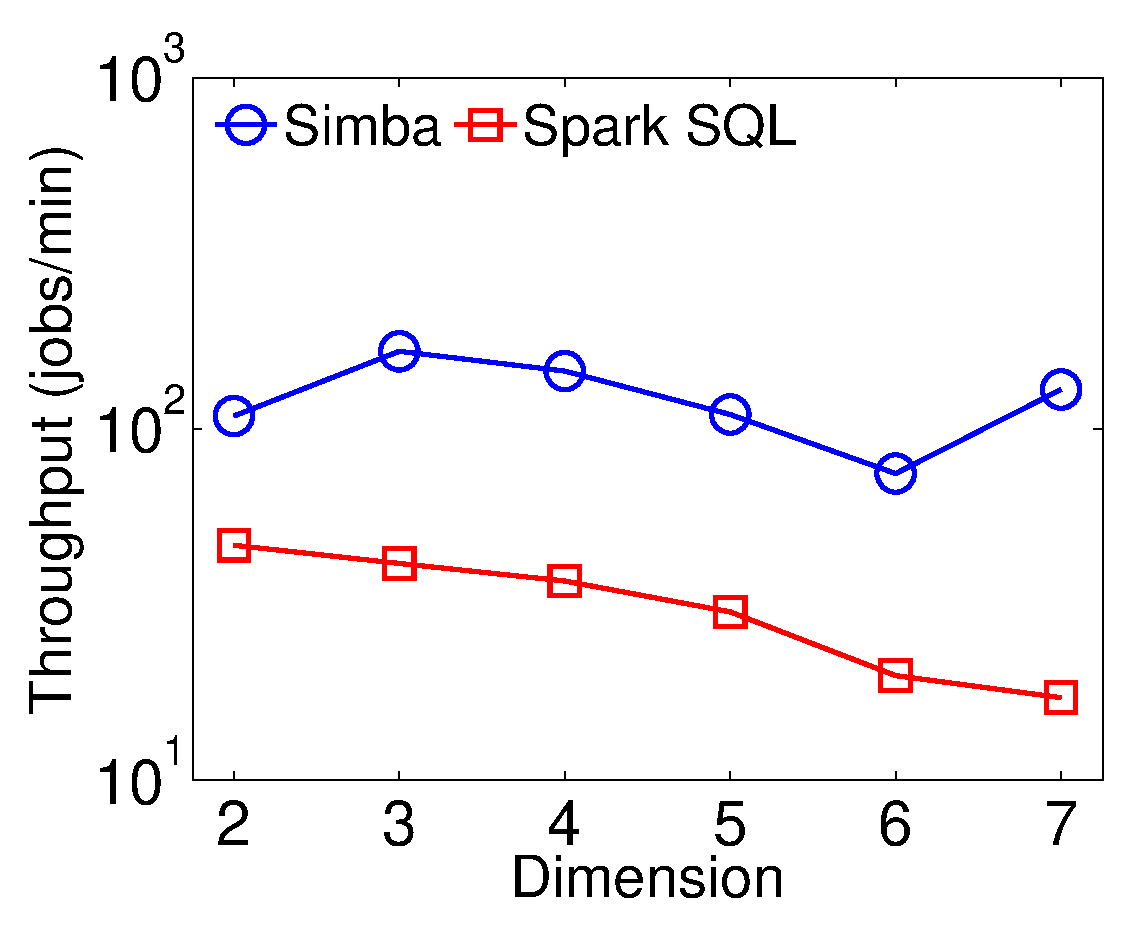
\includegraphics[width=1.55in]{figs/exp/gdelt_rect_dimension_throughput}
	%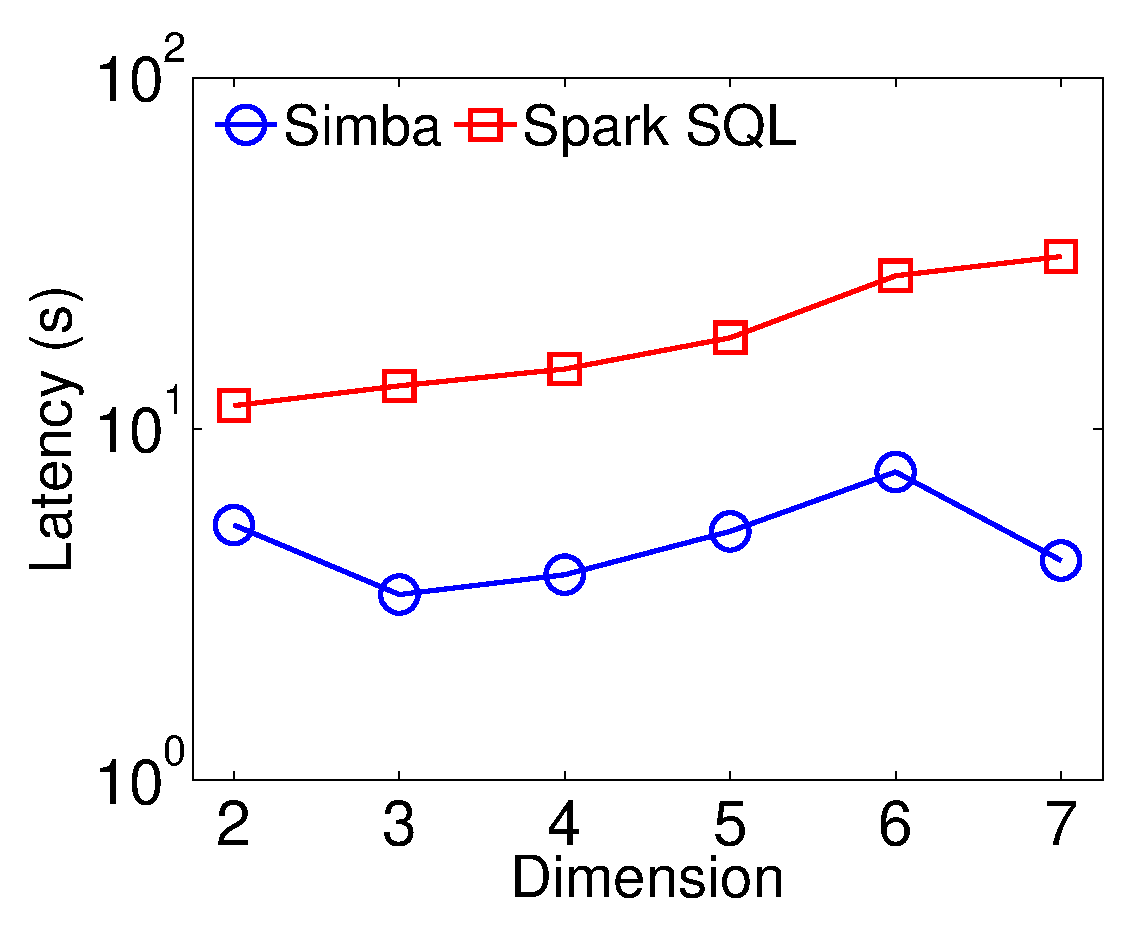
\includegraphics[width=1.55in]{figs/exp/gdelt_rect_dimension_latency}
	
	\caption{\small Range query performance vs. dimensionality on GDELT.}
	\label{fig:gdelt_rect_dimension}\vspace{-3mm}
\end{figure}

\begin{figure}[t]
	\centering
	% \subfigure[Synthetic]{
	% 	\label{fig:synthetic_knn_dimension}
	% 	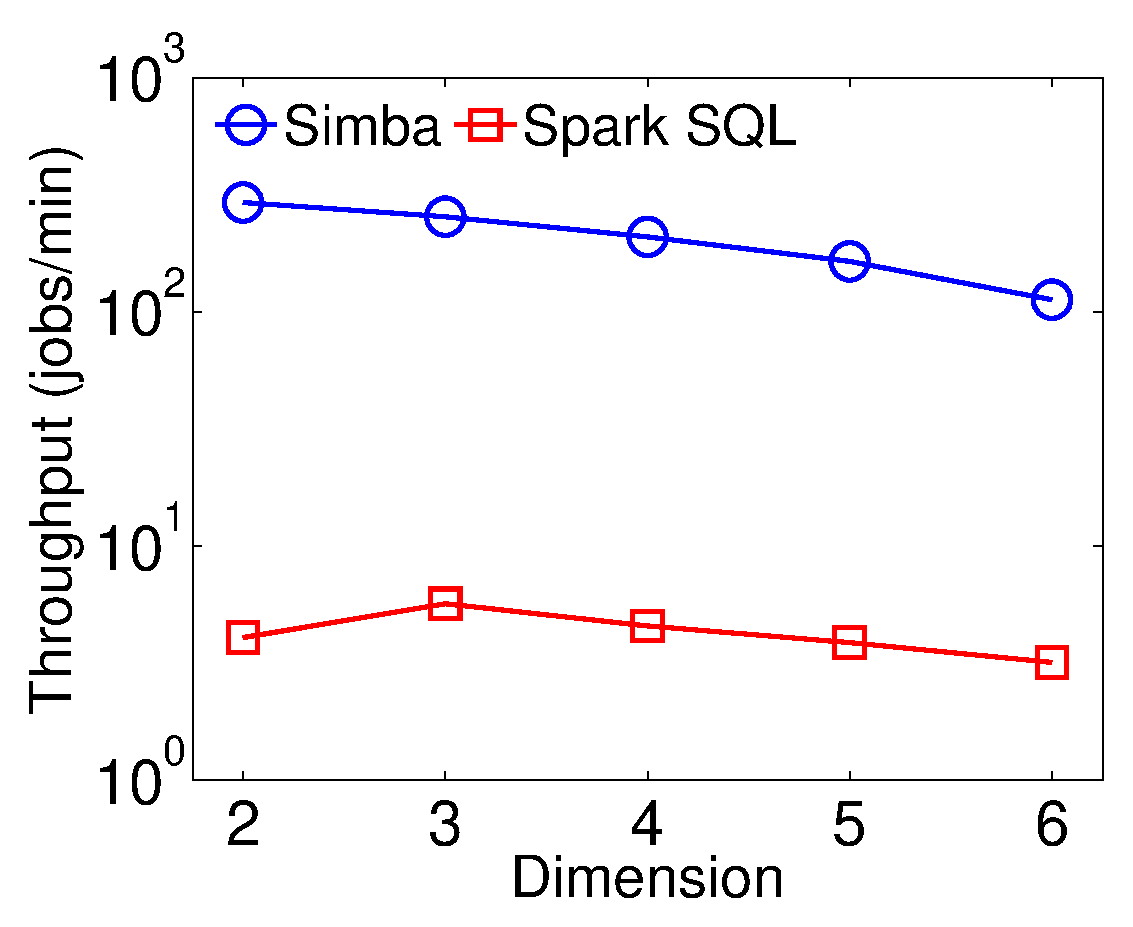
\includegraphics[width=1.55in]{figs/exp/gaussian700m_knn_dimension_throughput}
	% 	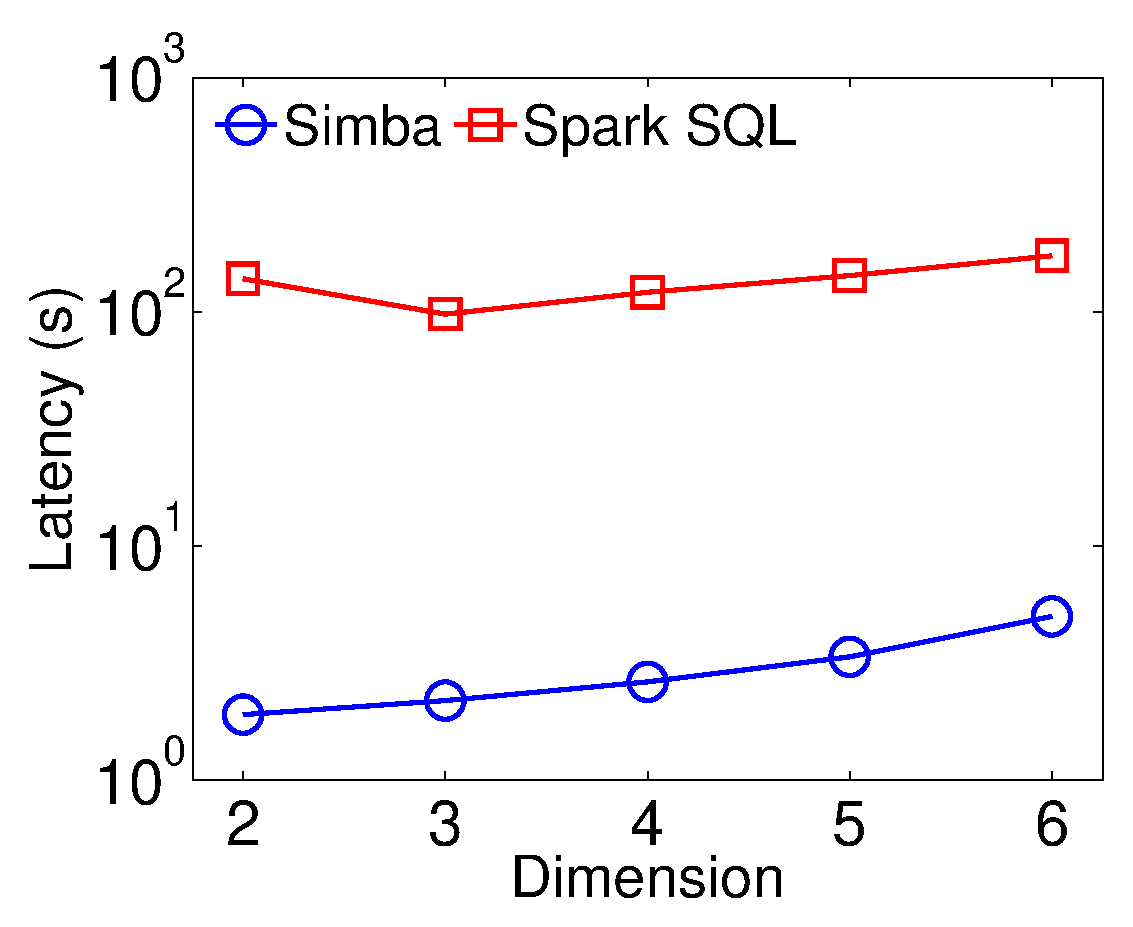
\includegraphics[width=1.55in]{figs/exp/gaussian700m_knn_dimension_latency}
	% }
	%\subfigure[GDELT]{
	%\label{fig:gdelt_knn_dimension}
	\subfigure[Throughput] {
		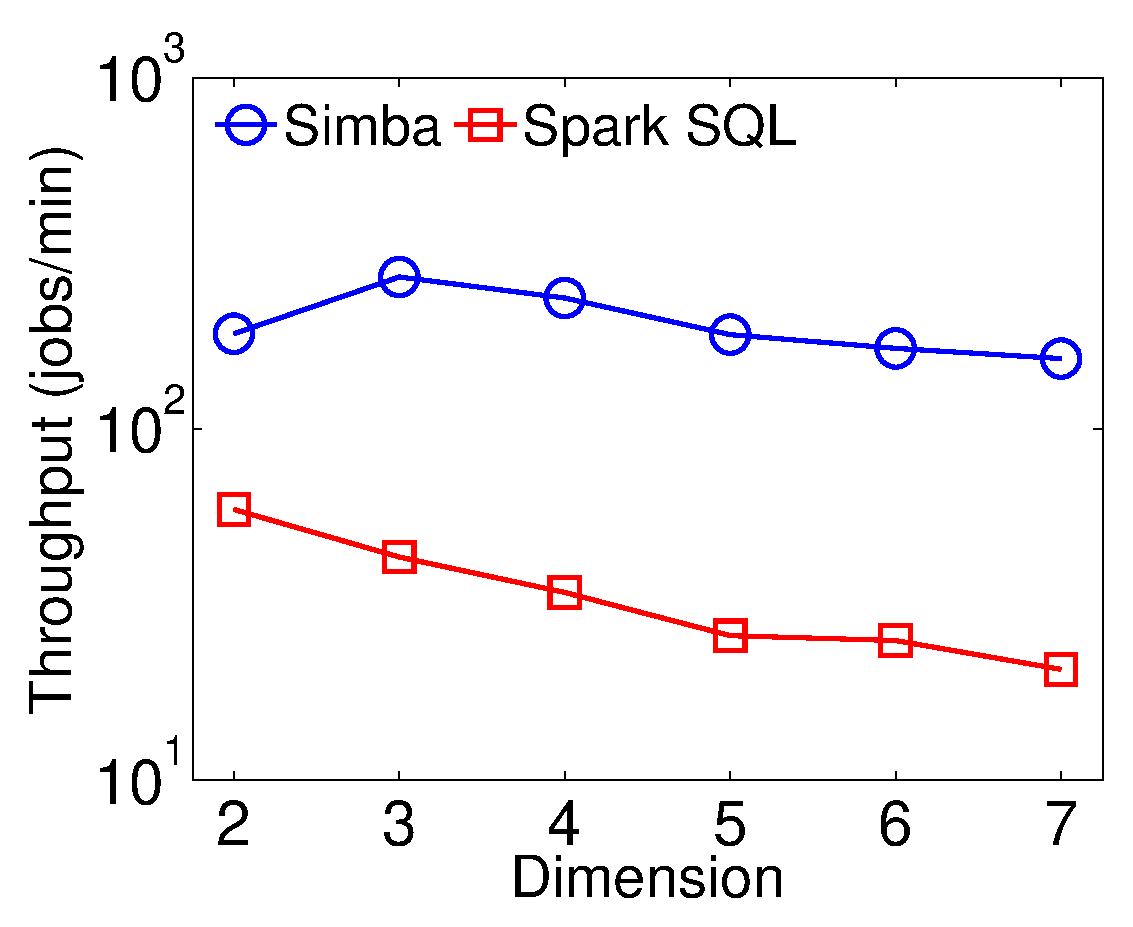
\includegraphics[width=1.55in]{figs/exp/gdelt_knn_dimension_throughput}
		\label{fig:gdelt_knn_dim_throughput}
	}
	\subfigure[Latency] {
		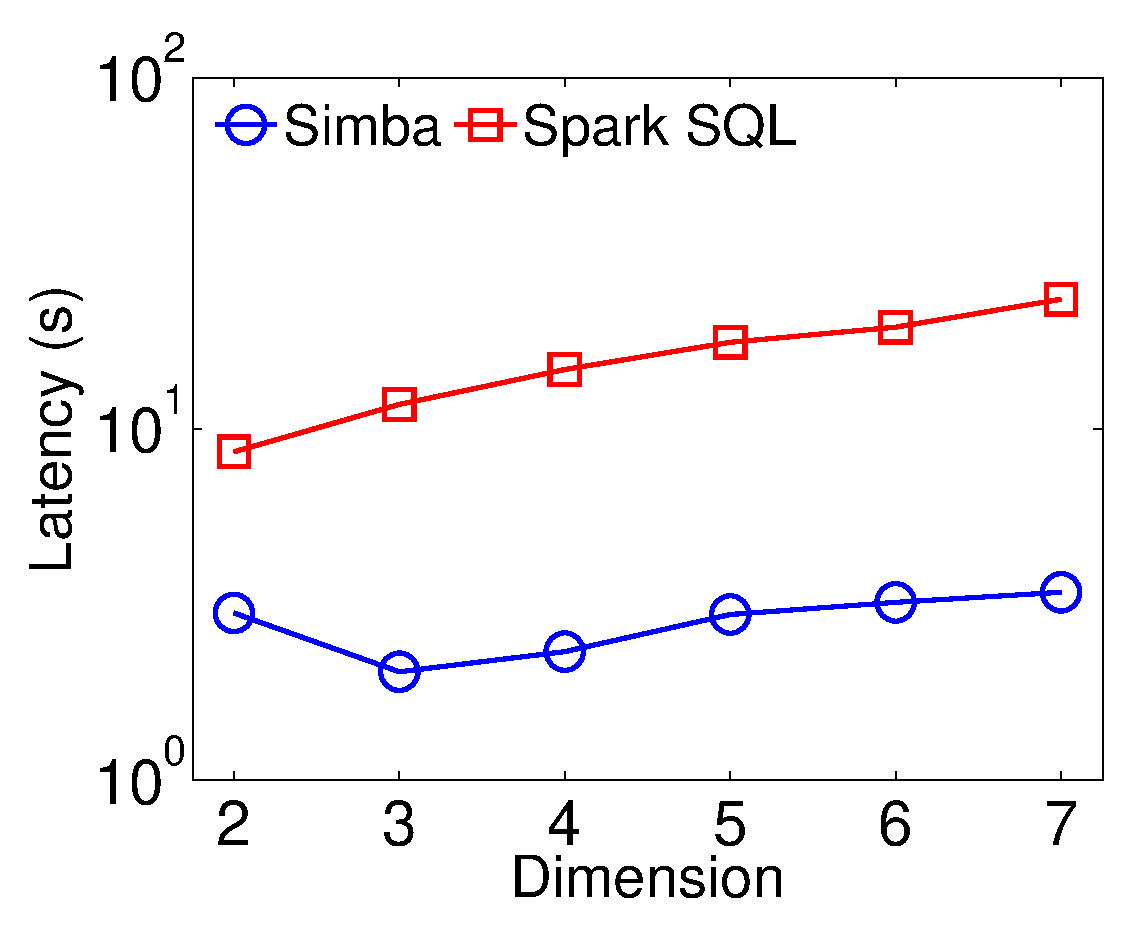
\includegraphics[width=1.55in]{figs/exp/gdelt_knn_dimension_latency}
		\label{fig:gdelt_knn_dim_latency}
	}
	%}\vspace{-1mm}
	\caption{\small $k$NN query performance vs. dimensionality on GDELT.}
	\label{fig:gdelt_knn_dimension}\vspace{-3mm}
\end{figure}

\begin{figure}[!t]
	\centering
	\subfigure[Distance join]{
		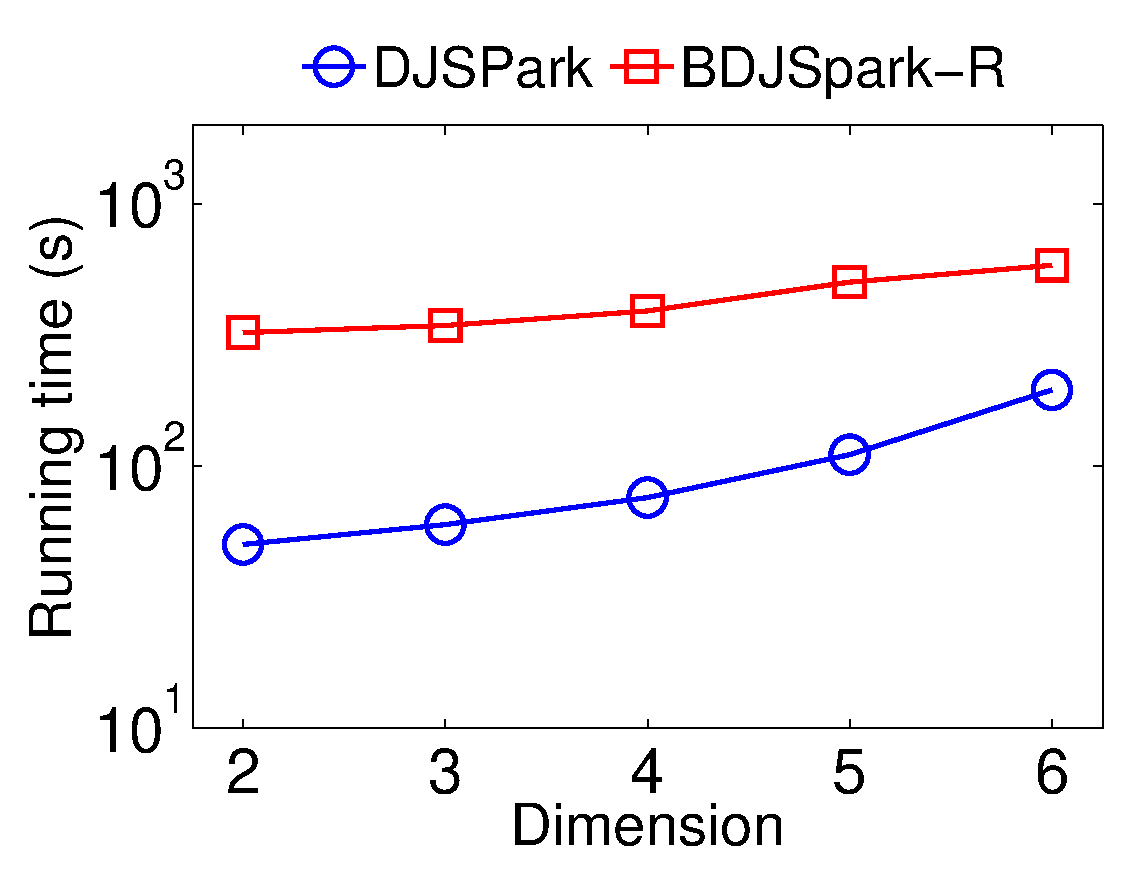
\includegraphics[width=1.55in]{figs/exp/osm_disj_dimension}
		\label{fig:synthetic_disj_dimension}}
	\subfigure[$k$NN join]{
		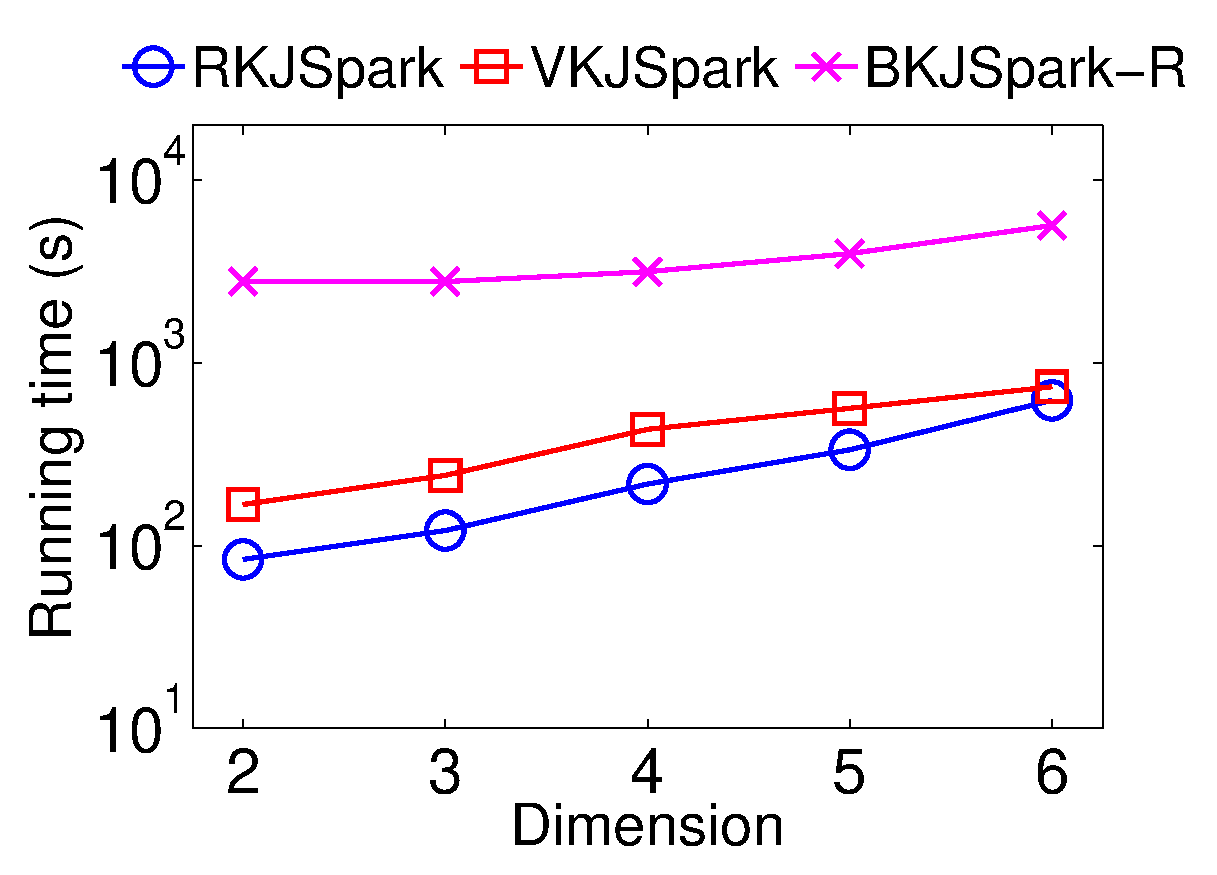
\includegraphics[width=1.55in]{figs/exp/osm_knnj_dimension}
		\label{fig:synthetic_knnj_dimension}}
	\caption{Join operations vs. dimensionality.}\vspace{-4mm}
	\label{fig:join_dim}
\end{figure}

\subsection{Support for Multi-Dimensions}
\label{sec:mdexp}
In this section, we evaluate the performance of \name and Spark SQL
when handling data in higher dimensions; note that other spatial
analytics systems, SpatialSpark, SpatialHadoop, and Hadoop GIS, {\em
  do not} support more than 2 dimensions.

For both range and $k$NN queries, as shown in Figures
\ref{fig:gdelt_rect_dimension} and \ref{fig:gdelt_knn_dimension}, both \name
and Spark SQL shows higher query latency and lower system throughput
using the GDELT data set, as dimensionality increases from $2$ to $6$.
But \name outperforms Spark SQL by 1-2 orders of magnitude in all cases.

% Figure \ref{fig:range_dim} shows how the number of dimensions
% influences range queries: On the synthetic RC dataset, \name and Spark
% SQL get slightly slower when the dimension number increases. On GDELT
% dataset, performance of \name is not stable since data distribution on
% different dimensions is not uniform. As to $k$NN queries shown in
% Figure \ref{fig:knn_dim}, performance on both data sets reduces
% steadily with the increasing of dimension number.  This is because the
% result sizes of $k$NN queries are fixed.


Figure \ref{fig:join_dim} shows the impact of dimensionality to the
join algorithms in \name, using two tables with 3 million records in
each table from the synthetic RC data set, when $d$ goes from $2$ to
$6$. The results show that the DJSpark and the RKJSpark algorithms
remain the best performance in all
dimensions. % From Figure \ref{fig:synthetic_disj_dimension}, we can observe
% that running time of BDJSpark-R grows slower than that of DJSpark and
% HDJSpark. The reason for this is the pruning power of the global join
% phase weakens with increasing of dimension number when the partition
% number is fixed. Similarly, BKJSpark-R grows slower than RKJSpark and
% VKJSpark (as shown in Figure \ref{fig:synthetic_knnj_dimension}) for
% the same reason. In addition, RKJSpark maintains comparable
% performance to VKJSpark on different dimension numbers.



%%% Local Variables:
%%% mode: latex
%%% TeX-master: "paper"
%%% End:
